\chapterimage{map.png}

\chapter{Arquitectura de Software}


\section{Fundamentos del Diseño Arquitectónico}

El diseño de arquitectura de software es la base fundamental para cualquier sistema de software complejo. Desafortunadamente, con frecuencia se realiza de manera ad hoc, si es que se realiza. Es nuestra convicción, basada en la experiencia, que tener una manera estructurada de realizar el diseño resulta en mejores resultados y más predecibles.

\subsection{La Necesidad de un Método Sistemático}

El diseño de arquitectura requiere un método sistemático que considere todos los aspectos relevantes necesarios para producir un diseño adecuado. Tal método debe proporcionar la guía necesaria para garantizar que los impulsores arquitectónicos (architectural drivers) sean satisfechos.

Para lograr este objetivo de manera efectiva y repetible, se necesita un método que guíe en la combinación e incorporación de conceptos de diseño reutilizables.

\subsection{Importancia del Diseño Arquitectónico}

Realizar un diseño arquitectónico adecuado es importante porque las decisiones de diseño tienen consecuencias significativas en diferentes puntos del ciclo de vida del proyecto:

\begin{itemize}
    \item Durante la fase de estimación, un diseño apropiado permitirá una mejor estimación de costos, alcance y cronograma.
    \item Durante el desarrollo, un diseño apropiado ayudará a evitar retrabajos posteriores y facilitará el desarrollo y despliegue.
    \item Una comprensión clara de lo que involucra el diseño arquitectónico es necesaria para gestionar mejor aspectos de la deuda técnica.
\end{itemize}


\subsection{Características de Calidad según ISO/IEC 9126 y el Modelo de McCall}

En ingeniería de sistemas y de requisitos, un requisito no funcional (NFR) es un requisito que especifica criterios que pueden ser utilizados para juzgar la operación de un sistema, en lugar de comportamientos específicos. Estos se contrastan con los requisitos funcionales que definen comportamientos o funciones específicas. El plan para implementar los requisitos funcionales se detalla en el diseño del sistema. El plan para implementar los requisitos no funcionales se detalla en la arquitectura del sistema, ya que generalmente son requisitos significativos a nivel arquitectónico.

En la arquitectura de software, los requisitos no funcionales se conocen como "características arquitectónicas". Es importante especificar los requisitos no funcionales de manera específica y medible.

\begin{itemize}
    \item \textbf{Funcionalidad}: Conjunto de atributos que afectan la existencia de un conjunto de funciones y sus propiedades especificadas. Incluye adecuación, exactitud, interoperabilidad, seguridad y cumplimiento funcional.
    \item \textbf{Fiabilidad}: Capacidad del software para mantener su nivel de rendimiento bajo condiciones establecidas durante un período de tiempo. Incluye madurez, tolerancia a fallos, recuperabilidad y cumplimiento de fiabilidad.
    \item \textbf{Usabilidad}: Esfuerzo necesario para el uso y la evaluación individual de dicho uso por un conjunto de usuarios. Incluye comprensibilidad, facilidad de aprendizaje, operabilidad y cumplimiento de usabilidad.
    \item \textbf{Eficiencia}: Relación entre el nivel de rendimiento del software y la cantidad de recursos utilizados bajo condiciones establecidas. Incluye comportamiento temporal, utilización de recursos y cumplimiento de eficiencia.
    \item \textbf{Mantenibilidad}: Esfuerzo necesario para realizar modificaciones especificadas. Incluye analizabilidad, capacidad de cambio, estabilidad, capacidad de prueba y cumplimiento de mantenibilidad.
    \item \textbf{Portabilidad}: Capacidad del software para ser transferido de un entorno a otro. Incluye adaptabilidad, instalabilidad, coexistencia, reemplazabilidad y cumplimiento de portabilidad.
\end{itemize}

\textbf{Modelo de Calidad de McCall (1977)}

El modelo de McCall se centra en tres perspectivas principales para evaluar la calidad del software:
\begin{figure}[H]
    \centering
    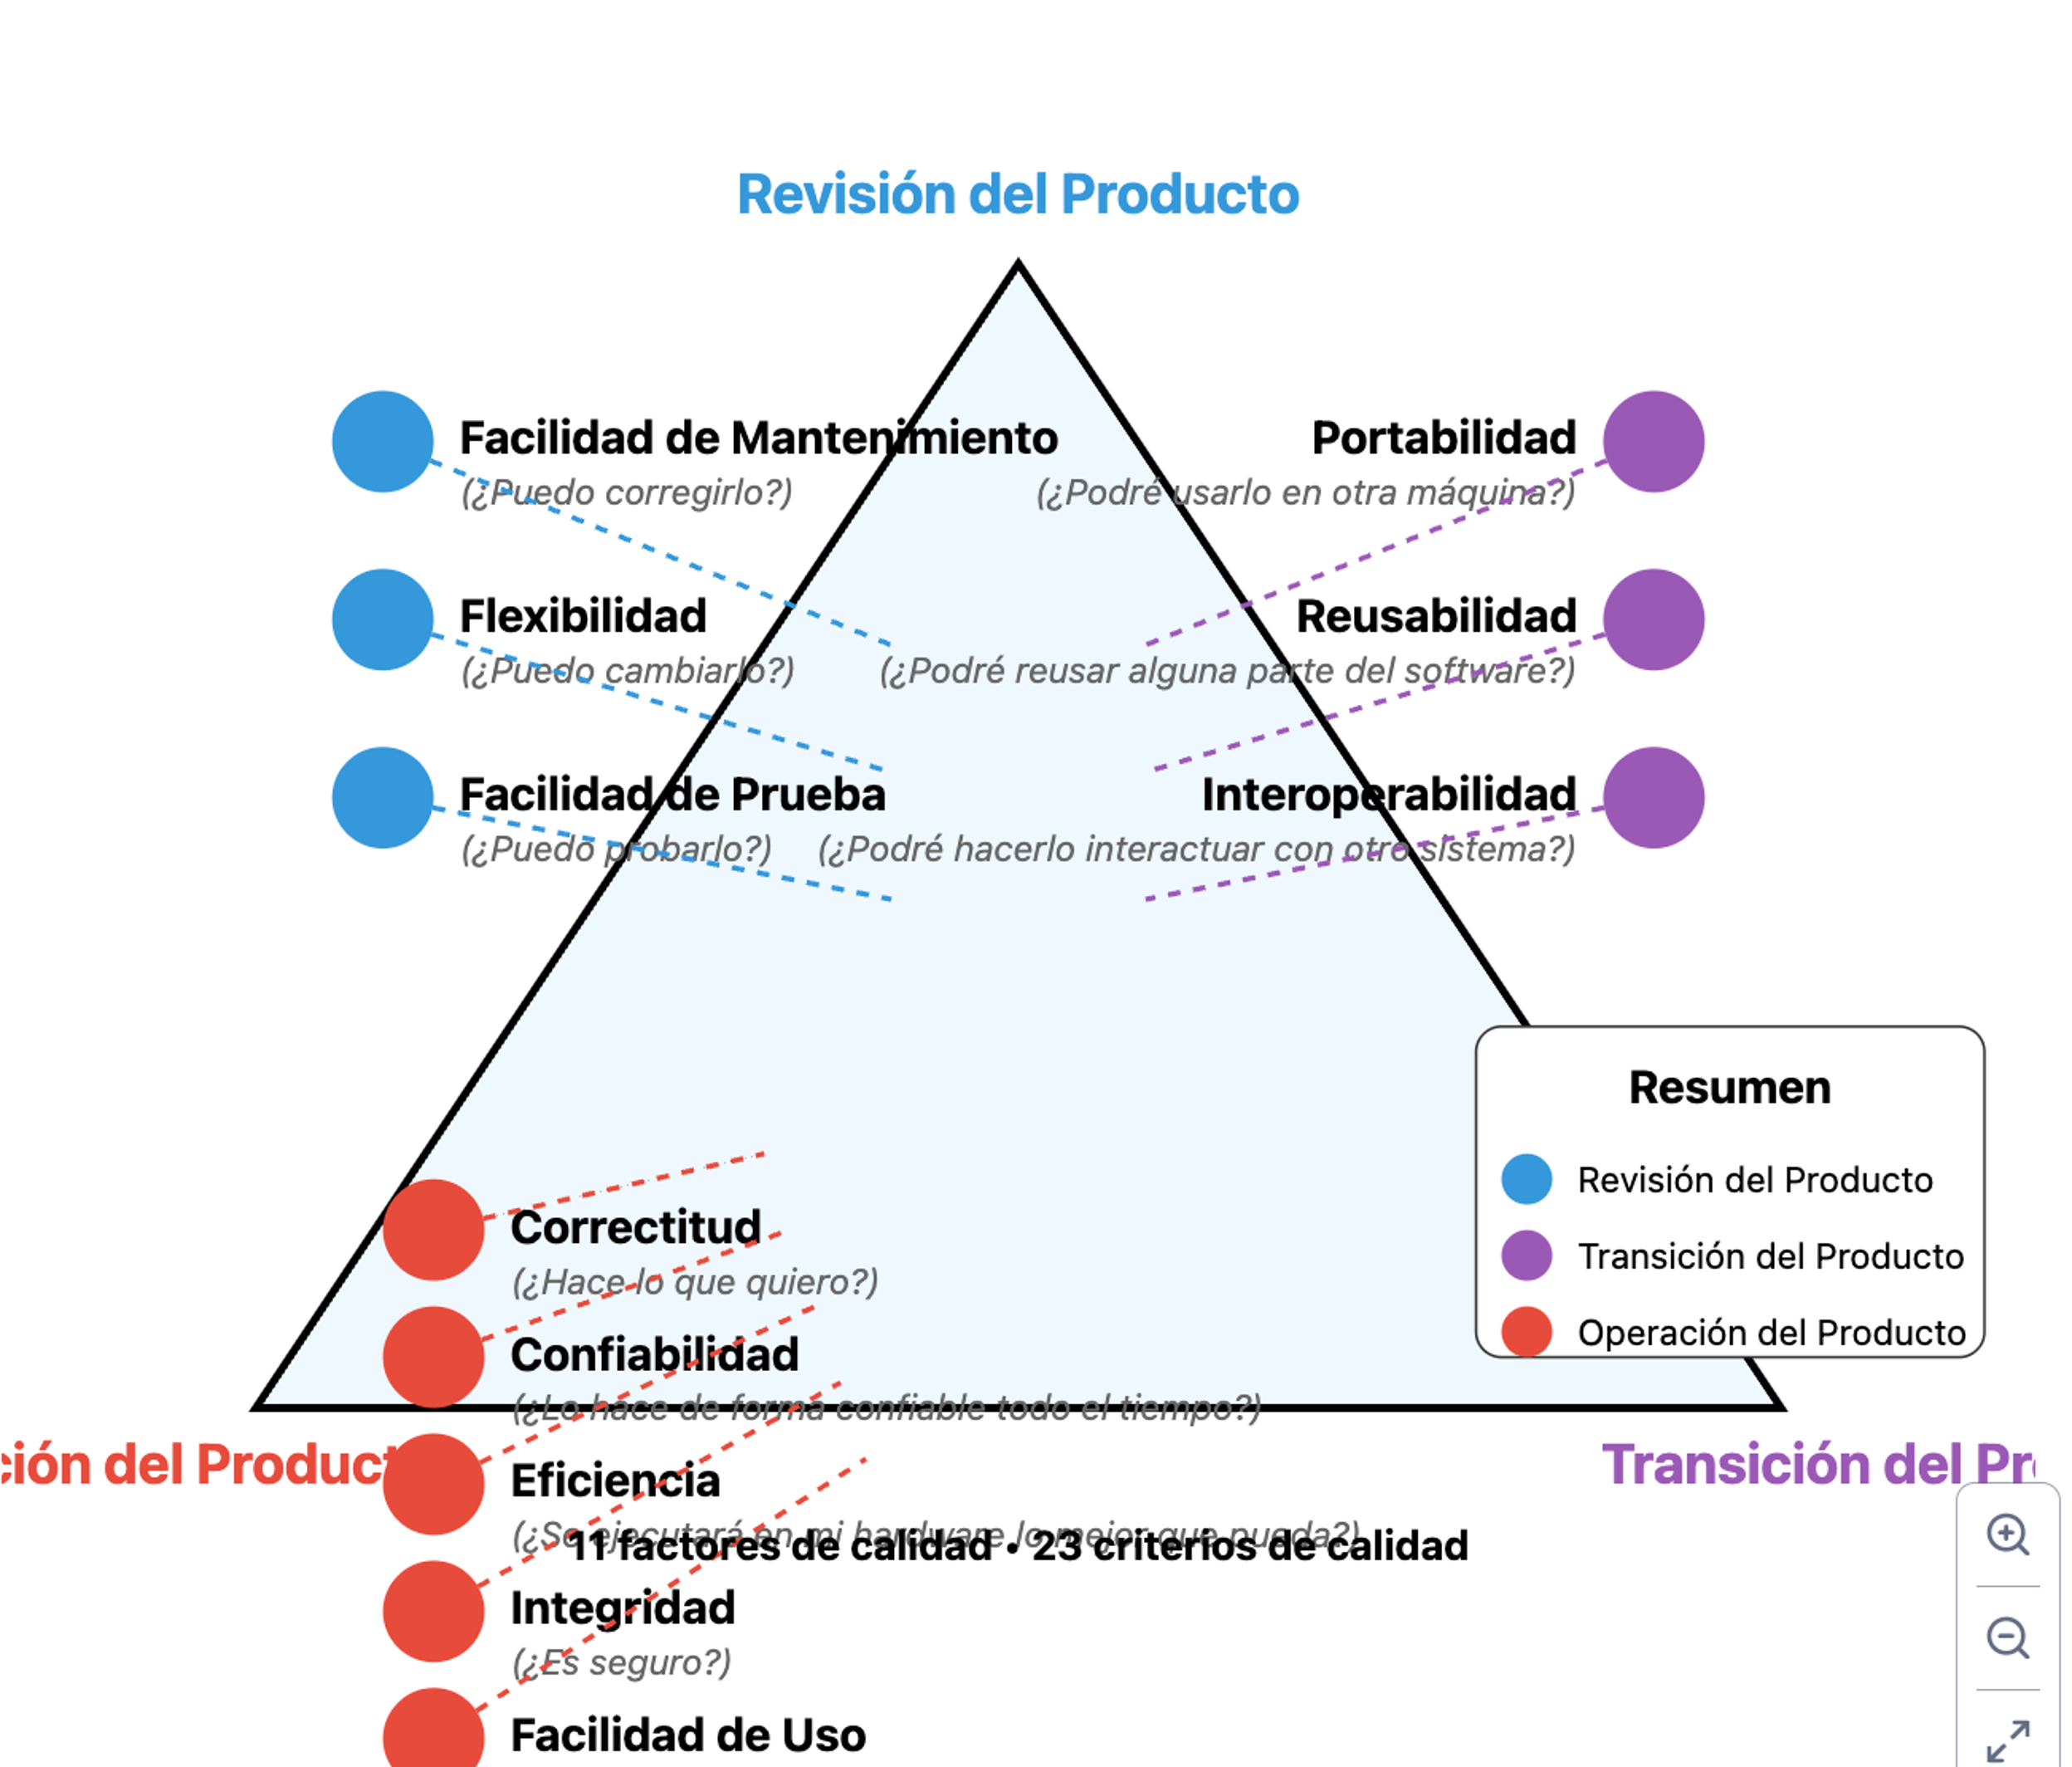
\includegraphics[width=0.8\textwidth]{Pictures/mccall.png}
    \caption{Modelo de Calidad de McCall}
    \label{fig:mccall}
\end{figure}

\begin{itemize}
    \item \textbf{Revisión del Producto}:
    \begin{itemize}
        \item Facilidad de Mantenimiento: ¿Puede corregirse el software fácilmente?
        \item Flexibilidad: ¿Puede cambiarse el software para adaptarse a nuevas necesidades?
        \item Facilidad de Prueba: ¿Puede probarse el software de manera efectiva?
    \end{itemize}
    \item \textbf{Transición del Producto}:
    \begin{itemize}
        \item Portabilidad: ¿Puede usarse el software en diferentes entornos?
        \item Reusabilidad: ¿Pueden reutilizarse partes del software en otros proyectos?
        \item Interoperabilidad: ¿Puede interactuar el software con otros sistemas?
    \end{itemize}
    \item \textbf{Operación del Producto}:
    \begin{itemize}
        \item Correctitud: ¿Hace el software lo que se espera?
        \item Confiabilidad: ¿Funciona el software de manera confiable?
        \item Eficiencia: ¿Utiliza el software los recursos de manera óptima?
        \item Integridad: ¿Es seguro el software?
        \item Facilidad de Uso: ¿Es fácil de usar el software?
    \end{itemize}
\end{itemize}

PD: se recomienda revisar la ISO25000 para un listado más exhaustivo de atributos de calidad.

\section{Conceptos de Diseño y Drivers Arquitectónicos}

Esta sección describe los conceptos de diseño y cómo se relacionan con los impulsores arquitectónicos, separando el diseño de la arquitectura de su evaluación.

\begin{itemize}
\item \textbf{Propósito del Diseño}: Definir el objetivo principal del diseño arquitectónico.
\item \textbf{Funcionalidad Primaria}: Describir las funciones esenciales que el sistema debe cumplir.
\item \textbf{Atributos de Calidad}: Detallar los atributos de calidad que guían las decisiones de diseño, como desempeño, seguridad, y usabilidad.
\item \textbf{Restricciones}: Enumerar las limitaciones que afectan el diseño, como restricciones tecnológicas o de presupuesto.
\item \textbf{Preocupaciones Arquitectónicas}: Identificar las preocupaciones clave que deben abordarse en el diseño.
\item \textbf{Drivers Arquitectónicos}: Especificar los impulsores arquitectónicos que influyen en las decisiones de diseño, como requisitos de negocio, necesidades de los usuarios y condiciones del entorno.
\end{itemize}





\subsection{El Proceso de Diseño Arquitectónico}

El diseño arquitectónico se lleva a cabo en una serie de rondas a lo largo del desarrollo de un proyecto de software. Cada ronda puede ocurrir dentro de un incremento del proyecto, como un sprint. Dentro de estas rondas, se realizan varias iteraciones de diseño. A continuación, se detallan los pasos del proceso de diseño arquitectónico con consejos, explicaciones y ejemplos específicos sobre cómo ejecutarlos:

\begin{enumerate}
    \item \textbf{Revisar las entradas del proceso de diseño:} 
    \begin{itemize}
        \item \textit{Descripción:} Identificar y analizar toda la información relevante que influirá en el diseño, como requisitos del cliente, restricciones tecnológicas y normativas.
        \item \textit{Consejo:} Asegúrate de tener una comprensión clara de los requisitos y limitaciones antes de proceder.
        \item \textit{Ejemplo:} Revisar los requisitos funcionales y no funcionales de una aplicación de comercio electrónico, como la necesidad de manejar 10,000 transacciones por día y cumplir con las normativas de protección de datos.
    \end{itemize}
    
    \item \textbf{Establecer el objetivo de la iteración seleccionando los impulsores:}
    \begin{itemize}
        \item \textit{Descripción:} Definir qué aspectos del sistema se mejorarán o desarrollarán en esta iteración, basándose en los impulsores arquitectónicos.
        \item \textit{Consejo:} Prioriza los impulsores que tengan el mayor impacto en los objetivos del proyecto.
        \item \textit{Ejemplo:} Seleccionar la mejora de la experiencia del usuario en el proceso de pago como objetivo principal de la iteración.
    \end{itemize}
    
    \item \textbf{Elegir uno o más elementos del sistema para refinar:}
    \begin{itemize}
        \item \textit{Descripción:} Seleccionar componentes específicos del sistema que requieren mejoras o ajustes.
        \item \textit{Consejo:} Considera la interdependencia entre componentes para evitar efectos negativos en el sistema.
        \item \textit{Ejemplo:} Decidir refinar el módulo de pago para reducir el tiempo de procesamiento y mejorar la seguridad.
    \end{itemize}
    
    \item \textbf{Seleccionar conceptos de diseño que satisfagan los impulsores seleccionados:}
    \begin{itemize}
        \item \textit{Descripción:} Identificar y aplicar principios de diseño que aborden los impulsores seleccionados.
        \item \textit{Consejo:} Evalúa diferentes enfoques de diseño y elige el que mejor se alinee con los objetivos del proyecto.
        \item \textit{Ejemplo:} Aplicar un diseño de microservicios para el módulo de pago que permita escalabilidad y actualizaciones independientes.
    \end{itemize}
    
    \item \textbf{Instanciar elementos arquitectónicos y definir interfaces:}
    \begin{itemize}
        \item \textit{Descripción:} Crear instancias de los elementos arquitectónicos y definir cómo interactuarán entre sí.
        \item \textit{Consejo:} Asegúrate de que las interfaces sean claras y bien documentadas para facilitar la integración.
        \item \textit{Ejemplo:} Definir interfaces API RESTful para el módulo de pago que permitan la comunicación con el sistema de inventario y el sistema de usuarios.
    \end{itemize}
    
    \item \textbf{Documentar vistas y decisiones de diseño:}
    \begin{itemize}
        \item \textit{Descripción:} Registrar las decisiones de diseño y las vistas arquitectónicas para referencia futura.
        \item \textit{Consejo:} Utiliza diagramas y descripciones detalladas para comunicar efectivamente el diseño a todos los interesados.
        \item \textit{Ejemplo:} Crear diagramas de componentes y secuencia que muestren cómo el módulo de pago interactúa con otros módulos del sistema de comercio electrónico.
    \end{itemize}
    
    \item \textbf{Realizar análisis del diseño actual:}
    \begin{itemize}
        \item \textit{Descripción:} Evaluar el diseño para identificar áreas de mejora y asegurar que cumple con los requisitos.
        \item \textit{Consejo:} Involucra a diferentes partes interesadas en el análisis para obtener una perspectiva completa.
        \item \textit{Ejemplo:} Realizar una revisión de diseño con el equipo de desarrollo y los stakeholders para asegurar que el módulo de pago cumple con los estándares de seguridad y rendimiento.
    \end{itemize}
\end{enumerate}


\color{blue}
\subsection{Caso de Estudio: Hospital Rural Integrado a la Ficha Clínica Nacional}

Este caso de estudio se centra en un hospital rural con limitaciones tecnológicas que se ha integrado recientemente a la ficha clínica nacional administrada por el MINSAL. El hospital cuenta con un sistema de información de agenda electrónica, notificaciones por SMS y WhatsApp, y un subsistema para la gestión de inventario de insumos médicos, agenda de pabellones, y un sistema de recursos humanos y finanzas.

\begin{itemize}
    \item \textbf{Propósito del Diseño}: Visualizar la arquitectura existente del hospital para comprender mejor los sistemas integrados y su interacción.
    \item \textbf{Funcionalidad Primaria}: Identificar y documentar las funciones esenciales de los sistemas actuales, como la gestión de citas, notificaciones, y administración de inventario y recursos.
    \item \textbf{Atributos de Calidad}: Evaluar la interoperabilidad, seguridad, y eficiencia de los sistemas existentes.
    \item \textbf{Restricciones}: Considerar las limitaciones tecnológicas del hospital y la falta de acceso al código fuente para realizar ingeniería inversa.
    \item \textbf{Preocupaciones Arquitectónicas}: Asegurar que la visualización de la arquitectura refleje con precisión la integración con la ficha clínica nacional y otros subsistemas.
    \item \textbf{Drivers Arquitectónicos}: Mejorar la comprensión de la arquitectura para facilitar futuras mejoras y asegurar el cumplimiento con las normativas del MINSAL.
\end{itemize}

%%%%%%%%%%%%%%
\subsubsection{Revisar las Entradas del Proceso de Diseño}

\begin{itemize}
    \item \textbf{Escenario 1: Gestión de Citas Médicas}
    \begin{itemize}
        \item \textbf{Requerimiento Funcional:} Permitir la programación y modificación de citas médicas.
        \item \textbf{Atributo de Calidad:} Disponibilidad
        \item \textbf{Métrica y Valores Esperados:} Sistema disponible 24/7, tiempo de inactividad menor a 1 hora por mes.
    \end{itemize}
    \item \textbf{Escenario 2: Notificaciones a Pacientes}
    \begin{itemize}
        \item \textbf{Requerimiento Funcional:} Enviar notificaciones por SMS y WhatsApp.
        \item \textbf{Atributo de Calidad:} Usabilidad
        \item \textbf{Métrica y Valores Esperados:} Configuración intuitiva, comprensión del 95% de los usuarios.
    \end{itemize}
    \item \textbf{Escenario 3: Gestión de Inventario de Insumos Médicos}
    \begin{itemize}
        \item \textbf{Requerimiento Funcional:} Controlar el stock y generar alertas de reposición.
        \item \textbf{Atributo de Calidad:} Fiabilidad
        \item \textbf{Métrica y Valores Esperados:} Actualización en tiempo real, precisión del 99%.
    \end{itemize}
    \item \textbf{Escenario 4: Acceso a la Ficha Clínica Nacional}
    \begin{itemize}
        \item \textbf{Requerimiento Funcional:} Integración con la ficha clínica nacional.
        \item \textbf{Atributo de Calidad:} Interoperabilidad
        \item \textbf{Métrica y Valores Esperados:} Integración sin errores, tiempo de respuesta menor a 2 segundos.
    \end{itemize}
    \item \textbf{Escenario 5: Sistema de Recursos Humanos y Finanzas}
    \begin{itemize}
        \item \textbf{Requerimiento Funcional:} Gestionar la nómina y recursos humanos.
        \item \textbf{Atributo de Calidad:} Mantenibilidad
        \item \textbf{Métrica y Valores Esperados:} Actualizaciones sin interrupciones, tiempo de implementación menor a 1 día.
    \end{itemize}
\end{itemize}
Estas son las funcionalidades que provee el sistema actualmente: 
\begin{itemize}
    \item RF1: El sistema permitirá la programación de citas médicas por parte del personal administrativo.
    \item RF2: El sistema permitirá la modificación de citas médicas ya programadas.
    \item RF3: El sistema permitirá la cancelación de citas médicas.
    \item RF4: El sistema enviará notificaciones por SMS a los pacientes para recordarles sus citas.
    \item RF5: El sistema enviará notificaciones por WhatsApp a los pacientes para recordarles sus citas.
    \item RF6: El sistema enviará notificaciones a los médicos sobre sus citas programadas.
    \item RF7: El sistema proporcionará un panel de control para que el personal administrativo gestione todas las citas.
    \item RF8: El sistema controlará el stock de insumos médicos.
    \item RF9: El sistema permitirá el acceso a la ficha clínica nacional para los médicos autorizados.
    \item RF10: El sistema gestionará la nómina del personal del hospital.
    \item RF11: El sistema permitirá la gestión de datos de los empleados, como horarios y permisos.
    \item RF12: El sistema debe integrarse con otros sistemas de salud para el intercambio de datos.
    \item RF13: Los datos deben encriptarse durante su tráfico y almacenamiento.
    \item RF14: El sistema debe requerir autenticación de usuario para acceder a sus funcionalidades.
    \item RF15: El sistema debe mantener logs detallados para auditoría y seguimiento de actividades.
    \item RF16: El sistema debe estar disponible 24/7 con un tiempo de inactividad menor a 1 hora por mes.
    \item RF17: La interfaz debe ser fácil de usar para el personal médico y administrativo.
    \item RF18: El sistema debe optimizar el uso de recursos para asegurar un rendimiento óptimo.
    \item RF19: El sistema debe generar alertas automáticas para la reposición de insumos médicos.
    \item RF20: El sistema debe permitir la adición de nuevos ítems y funcionalidades sin afectar el rendimiento.
    \item RF21: El sistema debe permitir la trazabilidad de todas las acciones realizadas por los usuarios.
\end{itemize}


Es crucial considerar las restricciones tecnológicas y normativas que pueden influir en el diseño del sistema. Entre estas restricciones se incluyen:

\begin{itemize}
    \item \textbf{Ley de Protección de Datos Personales de Chile:} Cumplimiento con la Ley N° 19.628 para proteger la información sensible de los pacientes.
    \item \textbf{Interoperabilidad de la Ficha Clínica Electrónica:} Asegurar que el sistema cumpla con las normativas de interoperabilidad establecidas por el Ministerio de Salud de Chile.
    \item \textbf{Limitaciones Tecnológicas:} En un hospital rural, existe una restricción tecnológica como la conectividad limitada a internet, lo que afectaría la capacidad de sincronización de datos en tiempo real.
\end{itemize}







%%%%%%%%
\subsubsection{Establecer el Objetivo de la Iteración Seleccionando los Impulsores}

\textbf{Descripción:} Definir qué aspectos del sistema del hospital rural se mejorarán o desarrollarán en esta iteración, basándose en los impulsores arquitectónicos identificados.

\textbf{Consejo:} Prioriza los impulsores que tengan el mayor impacto en los objetivos del proyecto, especialmente aquellos que mejoren la mantenibilidad y la visibilidad del sistema.

\textbf{Ejemplo:}
\begin{itemize}
    \item \textbf{Mejora de la Mantenibilidad:}
    \begin{itemize}
        \item \textit{Impulsor:} Reducir la complejidad del código y mejorar la documentación.
        \item \textit{Objetivo:} Facilitar el mantenimiento y la actualización del sistema, permitiendo cambios más rápidos y menos propensos a errores.
    \end{itemize}
    \item \textbf{Visibilización del Sistema:}
    \begin{itemize}
        \item \textit{Impulsor:} Crear una representación clara de la arquitectura actual.
        \item \textit{Objetivo:} Documentar la arquitectura, identificando componentes clave y sus interacciones.
    \end{itemize}
    \item \textbf{Mejora de la Interoperabilidad:}
    \begin{itemize}
        \item \textit{Impulsor:} Asegurar que el sistema se integre eficazmente con otros sistemas de salud.
        \item \textit{Objetivo:} Mejorar la capacidad del sistema para comunicarse con la ficha clínica nacional y otros sistemas hospitalarios.
    \end{itemize}
\end{itemize}


\subsubsection{Elegir uno o más Elementos del Sistema para Refinar}
% Aquí se detallarán los pasos para elegir elementos del sistema a refinar.

% \item \textbf{Elegir uno o más elementos del sistema para refinar:}
% \begin{itemize}
%     \item \textit{Descripción:} Seleccionar componentes específicos del sistema que requieren mejoras o ajustes.
%     \item \textit{Consejo:} Considera la interdependencia entre componentes para evitar efectos negativos en el sistema.
%     \item \textit{Ejemplo:} Decidir refinar el módulo de pago para reducir el tiempo de procesamiento y mejorar la seguridad.
% \end{itemize}
Refinaremos interoperabilidad y disponibilidad con sistemas externos. 

El siguiente diagrama muestra el despliegue del sistema dada la instalación actual, no incluyendo los subsistemas o componentes existentes para recursos humanos, finanzas, entre otros.

\begin{figure}[h]
\centering
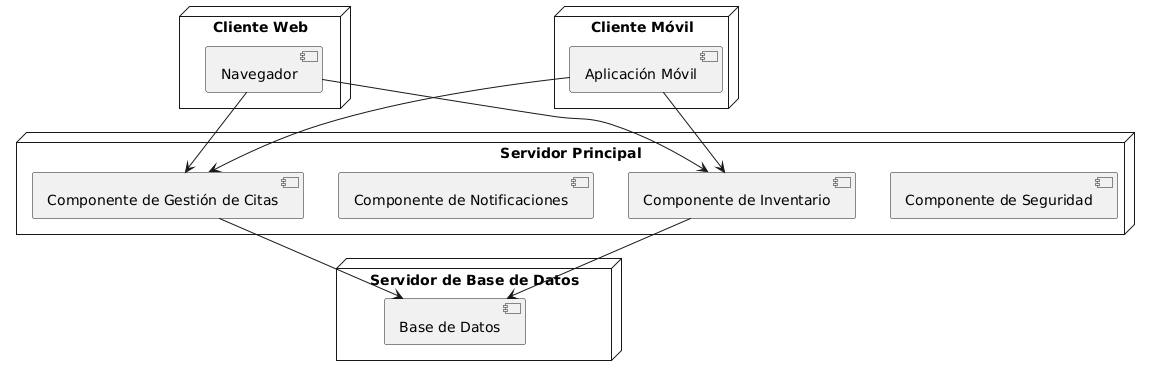
\includegraphics[width=\textwidth]{diagramadespliegue.png}
\caption{Diagrama de Despliegue del Sistema Completo}
\label{fig:complete_deployment_diagram}
\end{figure}


\begin{table}[h]
    \centering
    \begin{tabular}{|l|p{10cm}|}
    \hline
    \textbf{Escenario} & \textbf{Requerimientos Funcionales} \\ \hline
    \textbf{Gestión de Citas Médicas} & 
    \begin{itemize}
        \item RF1: El sistema permitirá la programación de citas médicas por parte del personal administrativo.
        \item RF2: El sistema permitirá la modificación de citas médicas ya programadas.
        \item RF3: El sistema permitirá la cancelación de citas médicas.
    \end{itemize} \\ \hline
    \textbf{Notificaciones a Pacientes*} & 
    \begin{itemize}
        \item RF4: El sistema enviará notificaciones por SMS a los pacientes para recordarles sus citas.
        \item RF5: El sistema enviará notificaciones por WhatsApp a los pacientes para recordarles sus citas.
        \item RF6: El sistema enviará notificaciones a los médicos sobre sus citas programadas.
    \end{itemize} \\ \hline
    \textbf{Gestión de Inventario de Insumos Médicos} & 
    \begin{itemize}
        \item RF8: El sistema controlará el stock de insumos médicos.
        \item RF19: El sistema debe generar alertas automáticas para la reposición de insumos médicos.
    \end{itemize} \\ \hline
    \textbf{Acceso a la Ficha Clínica Nacional} & 
    \begin{itemize}
        \item RF9: El sistema permitirá el acceso a la ficha clínica nacional para los médicos autorizados.
        \item RF12: El sistema debe integrarse con otros sistemas de salud para el intercambio de datos.
    \end{itemize} \\ \hline
    \textbf{Sistema de Recursos Humanos y Finanzas} & 
    \begin{itemize}
        \item RF10: El sistema gestionará la nómina del personal del hospital.
        \item RF11: El sistema permitirá la gestión de datos de los empleados, como horarios y permisos.
    \end{itemize} \\ \hline
    \end{tabular}
    \caption{Cruce de Escenarios con Requerimientos Funcionales}
    \label{tab:escenarios_requerimientos}
    \end{table}

Dijimos \textbf{Mejora de la Mantenibilidad}, y \textbf{Mejora de la Interoperabilidad} y el escenario  \textbf{Acceso a la Ficha Clínica Nacional} - RF9: El sistema permitirá el acceso a la ficha clínica nacional para los médicos autorizados. Para eso lo primero es crear un escenario detallado que nos servirá para una prueba de aceptación: 

\textbf{Escenario Detallado: Acceso a la Ficha Clínica Nacional}

\textbf{Contexto:} En un hospital rural, un médico está atendiendo a un paciente que ha sido derivado desde otro centro de salud. Durante la consulta, el médico necesita acceder a la ficha clínica nacional para revisar el historial médico del paciente, incluyendo diagnósticos previos, tratamientos y alergias conocidas. Este acceso es crucial para tomar decisiones informadas sobre el tratamiento actual del paciente.

\textbf{Requerimiento Funcional:} RF9: El sistema permitirá el acceso a la ficha clínica nacional para los médicos autorizados.

\textbf{Atributos de Calidad:}
\begin{itemize}
    \item \textbf{Interoperabilidad:} El sistema debe integrarse sin problemas con la ficha clínica nacional.
    \item \textbf{Seguridad:} El acceso debe ser seguro, garantizando la protección de los datos del paciente.
    \item \textbf{Disponibilidad:} El sistema debe estar disponible 24/7 para asegurar que los médicos puedan acceder a la información cuando sea necesario.
\end{itemize}

\textbf{Métrica y Valores Esperados:}
\begin{itemize}
    \item Tiempo de respuesta para acceder a la ficha clínica: menos de 2 segundos.
    \item Cumplimiento con las normativas de protección de datos personales.
\end{itemize}


\begin{figure}[h]
    \centering
    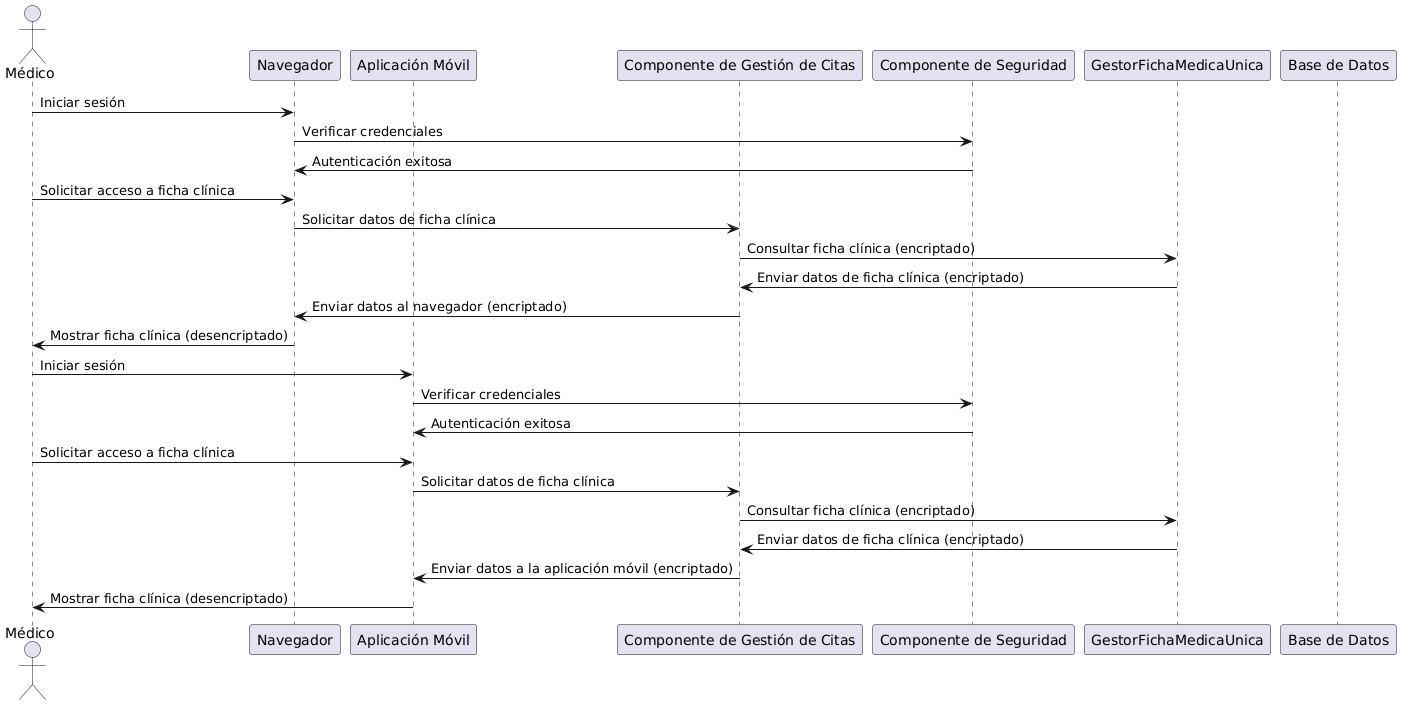
\includegraphics[width=\textwidth]{diagramasecuencia.png}
    \caption{Diagrama de Secuencia para el Escenario de Acceso a la Ficha Clínica Nacional}
    \label{fig:diagrama_secuencia}
\end{figure}
Ver más detalles en las slides de cómo ir verificando que si se cumple o no o si se debe seguir iterando. 

\subsubsection{Seleccionar Conceptos de Diseño que Satisfagan los Impulsores Seleccionados}
% Aquí se detallarán los pasos para seleccionar conceptos de diseño.

% \item \textbf{Seleccionar conceptos de diseño que satisfagan los impulsores seleccionados:}
% \begin{itemize}
%     \item \textit{Descripción:} Identificar y aplicar principios de diseño que aborden los impulsores seleccionados.
%     \item \textit{Consejo:} Evalúa diferentes enfoques de diseño y elige el que mejor se alinee con los objetivos del proyecto.
%     \item \textit{Ejemplo:} Aplicar un diseño de microservicios para el módulo de pago que permita escalabilidad y actualizaciones independientes.
% \end{itemize}

\subsubsection{Seleccionar Conceptos de Diseño que Satisfagan los Impulsores Seleccionados}

Dado los drivers arquitectónicos identificados, que incluyen la mejora de la mantenibilidad, la mejora de la interoperabilidad y el acceso a la ficha clínica nacional, hemos seleccionado un concepto de diseño que se enfoca en la redundancia, alta disponibilidad e interoperabilidad, adaptado a las limitaciones de un hospital rural con sistemas antiguos.

\textbf{Drivers Arquitectónicos:}
\begin{itemize}
    \item \textbf{Mejora de la Mantenibilidad:} Asegurar que el sistema pueda ser corregido y actualizado fácilmente, incluso con infraestructura antigua.
    \item \textbf{Mejora de la Interoperabilidad:} Garantizar que el sistema pueda interactuar sin problemas con otros sistemas, como la ficha clínica nacional proporcionada por el gobierno.
    \item \textbf{Acceso a la Ficha Clínica Nacional:} Permitir a los médicos autorizados acceder a la ficha clínica nacional de manera segura y eficiente.
\end{itemize}

Para abordar estos drivers, el gobierno ha adoptado un diseño que maximiza el uso de la infraestructura existente, integrando servicios gubernamentales para la ficha médica. Se ha implementado redundancia y alta disponibilidad mediante configuraciones de respaldo y sistemas de failover, asegurando que el sistema esté siempre disponible y pueda manejar fallos sin interrumpir el servicio.

\textbf{Nuevos Diagramas:}

\begin{figure}[h]
    \centering
    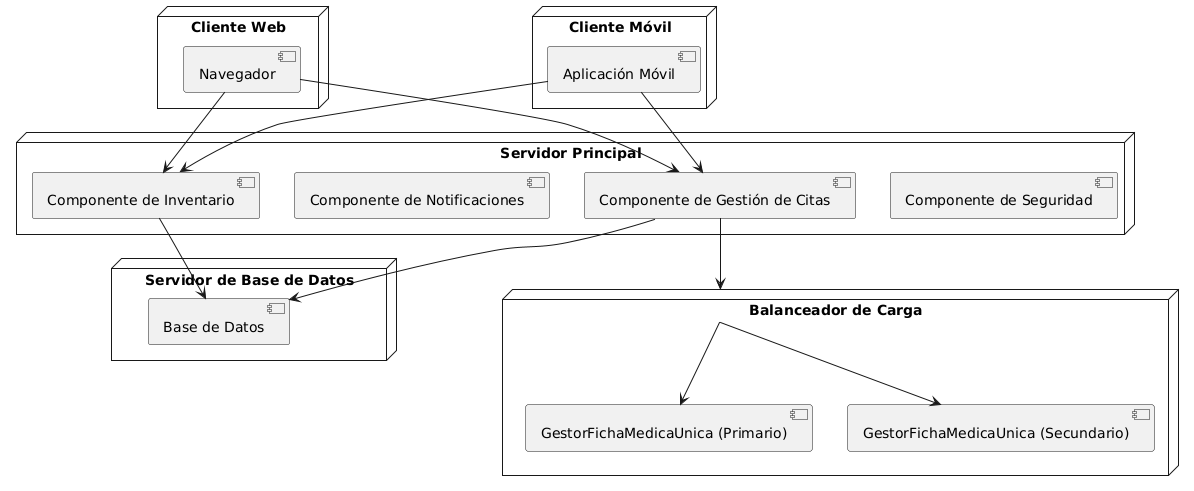
\includegraphics[width=\textwidth]{diagramadespliegue2.png}
    \caption{Diagrama de Despliegue con Alta Disponibilidad e Interoperabilidad}
    \label{fig:diagrama_despliegue2}
\end{figure}

El \textbf{Diagrama de Despliegue} muestra cómo los componentes del sistema están distribuidos en la infraestructura existente del hospital, utilizando servidores de respaldo para asegurar alta disponibilidad. Cada componente crítico tiene un sistema de failover, lo que permite que el sistema continúe funcionando incluso si uno de los servidores falla. Además, se utilizan configuraciones de red para asegurar que las solicitudes se redirijan adecuadamente en caso de fallos.

\begin{figure}[h]
    \centering
    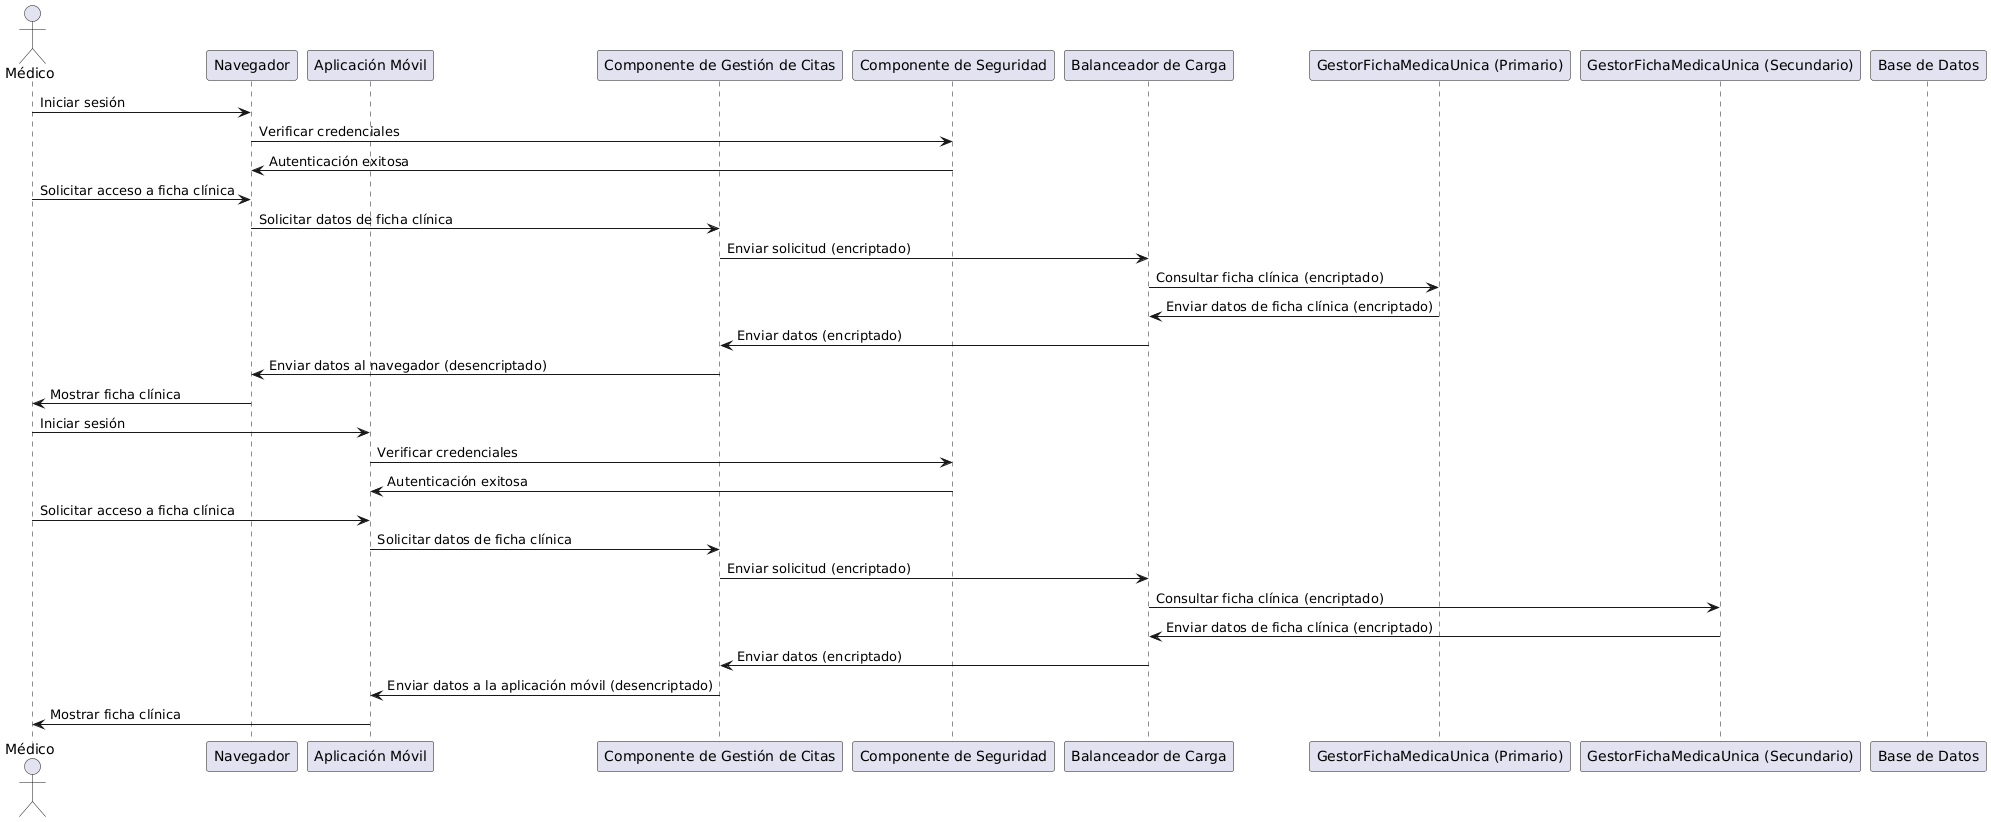
\includegraphics[width=\textwidth]{diagramasecuencia2.png}
    \caption{Diagrama de Secuencia para el Escenario de Acceso a la Ficha Clínica Nacional con Alta Disponibilidad}
    \label{fig:diagrama_secuencia2}
\end{figure}

El \textbf{Diagrama de Secuencia} actualizado muestra el flujo de interacción entre los componentes del sistema durante el acceso a la ficha clínica nacional. Este diagrama destaca cómo se maneja la redundancia y la alta disponibilidad en el proceso. Si un componente falla, el sistema redirige automáticamente la solicitud a un sistema de respaldo, asegurando que el acceso a la ficha clínica no se vea interrumpido.

Estos nuevos diseños no solo cubren los drivers arquitectónicos identificados, sino que también mejoran la resiliencia y la eficiencia del sistema, asegurando que los médicos puedan acceder a la información crítica del paciente en todo momento, incluso con las limitaciones de un entorno rural.


Para asegurar la integridad y confidencialidad de los datos en sistemas de información, se han considerado varias alternativas tecnológicas. A continuación, se presentan algunas de las opciones más relevantes:

\textbf{1. Uso de X-Road de Estonia:}
X-Road es una solución de intercambio de datos segura y escalable utilizada en Estonia. Permite la comunicación segura entre diferentes sistemas de información, garantizando la integridad y confidencialidad de los datos. Implementar X-Road podría proporcionar una capa adicional de seguridad y asegurar que los datos intercambiados entre diferentes entidades sean protegidos contra accesos no autorizados.

\textbf{2. Contratos Inteligentes con Neuroledger:}
Neuroledger es una plataforma que utiliza contratos inteligentes para asegurar la integridad de los datos. Los contratos inteligentes pueden verificar automáticamente la autenticidad de los datos y asegurar que no hayan sido alterados. Esta solución podría ser implementada para garantizar que los datos sean confiables y estén protegidos contra manipulaciones.

\textbf{3. Hashing de Datos:}
Una solución más sencilla podría ser el uso de hashes para verificar la integridad de los datos. Cada vez que se intercambian datos entre entidades, se podría generar un hash que se verifique en ambos extremos. Aunque esta solución es más casera, puede ser efectiva para asegurar que los datos no hayan sido alterados durante la transmisión.

\textbf{4. Encriptación de Datos:}
Para asegurar la confidencialidad de los datos, es esencial implementar encriptación. Los datos sensibles deben ser encriptados tanto en tránsito como en reposo. Esto asegurará que, incluso si los datos son interceptados, no puedan ser leídos por personas no autorizadas.

\textbf{5. Autenticación y Autorización:}
No se ha discutido en detalle cómo se manejará la autenticación y autorización en los sistemas de información. Es crucial explorar opciones como OAuth 2.0 y OpenID Connect para asegurar que solo usuarios autorizados puedan acceder a los datos. OAuth 2.0 proporciona un marco para la autorización segura, mientras que OpenID Connect añade una capa de autenticación, permitiendo verificar la identidad de los usuarios.

\textbf{Tarea para los Alumnos:}
Se recomienda a los alumnos investigar más a fondo estas alternativas de seguridad como una tarea que apoya la nota de participación y compartirla en el foro. Deberán buscar artículos en Medium  para evaluar las ventajas y desventajas de cada opción y proponer una solución que mejor se adapte a las necesidades de los sistemas de información y las limitaciones del entorno en el que se implementen.







\subsubsection{Instanciar Elementos Arquitectónicos y Definir Interfaces}
% Aquí se detallarán los pasos para instanciar elementos arquitectónicos.

% \item \textbf{Instanciar elementos arquitectónicos y definir interfaces:}
% \begin{itemize}
%     \item \textit{Descripción:} Crear instancias de los elementos arquitectónicos y definir cómo interactuarán entre sí.
%     \item \textit{Consejo:} Asegúrate de que las interfaces sean claras y bien documentadas para facilitar la integración.
%     \item \textit{Ejemplo:} Definir interfaces API RESTful para el módulo de pago que permitan la comunicación con el sistema de inventario y el sistema de usuarios.
% \end{itemize}

\textbf{Interfaces Propuestas:}

\begin{itemize}
    \item \textbf{Interface de Gestión de Citas:}
    \begin{itemize}
        \item \textbf{Método:} \texttt{updateAppointment}
        \item \textbf{Parámetros:} Identificador de cita, nueva fecha y hora, detalles del paciente.
        \item \textbf{Retorno:} \texttt{True} si la actualización es exitosa.
        \item \textbf{Excepciones:} \texttt{AppointmentUpdateException} si la actualización falla.
    \end{itemize}
    \item \textbf{Interface de Notificaciones:}
    \begin{itemize}
        \item \textbf{Método:} \texttt{sendNotification}
        \item \textbf{Parámetros:} Identificador del paciente, tipo de notificación (SMS, WhatsApp), mensaje.
        \item \textbf{Retorno:} \texttt{True} si la notificación se envía correctamente.
        \item \textbf{Excepciones:} \texttt{NotificationException} si el envío falla.
    \end{itemize}
    \item \textbf{Interface de Inventario:}
    \begin{itemize}
        \item \textbf{Método:} \texttt{updateStock}
        \item \textbf{Parámetros:} Identificador de insumo, cantidad, fecha de actualización.
        \item \textbf{Retorno:} \texttt{True} si la actualización es exitosa.
        \item \textbf{Excepciones:} \texttt{StockUpdateException} si la actualización falla.
    \end{itemize}
\end{itemize}









\subsubsection{Documentar Vistas y Decisiones de Diseño}
% Aquí se detallarán los pasos para documentar vistas y decisiones de diseño.
% \item \textbf{Documentar vistas y decisiones de diseño:}
% \begin{itemize}
%     \item \textit{Descripción:} Registrar las decisiones de diseño y las vistas arquitectónicas para referencia futura.
%     \item \textit{Consejo:} Utiliza diagramas y descripciones detalladas para comunicar efectivamente el diseño a todos los interesados.
%     \item \textit{Ejemplo:} Crear diagramas de componentes y secuencia que muestren cómo el módulo de pago interactúa con otros módulos del sistema de comercio electrónico.
% \end{itemize}


Las vistas de la arquitectura se dividen en varias categorías, cada una enfocada en un aspecto particular del sistema:

\textbf{Vista de Componentes y Conectores:}
\begin{itemize}
    \item \textbf{Propósito:} Mostrar los componentes principales del sistema y cómo interactúan.
    \item \textbf{Elementos:} componentes, conectores, protocolos de comunicación.
    \item \textbf{Beneficios:} Facilita el análisis de interacción y comunicación entre componentes.
\end{itemize}

\textbf{Vista de Módulos:}
\begin{itemize}
    \item \textbf{Propósito:} Describir la organización del software en módulos y sus relaciones.
    \item \textbf{Elementos:} Módulos, submódulos, dependencias.
    \item \textbf{Beneficios:} Ayuda en la planificación del desarrollo y la asignación de tareas.
\end{itemize}

\textbf{Vista de Despliegue:}
\begin{itemize}
    \item \textbf{Propósito:} Representar cómo el sistema se distribuye en la infraestructura física.
    \item \textbf{Elementos:} Servidores, redes, dispositivos.
    \item \textbf{Beneficios:} Permite evaluar la disponibilidad y redundancia del sistema.
\end{itemize}

\textbf{Vista de Ejecución:}
\begin{itemize}
    \item \textbf{Propósito:} Mostrar cómo se comporta el sistema durante la ejecución.
    \item \textbf{Elementos:} Procesos, hilos, interacciones en tiempo real.
    \item \textbf{Beneficios:} Ayuda a identificar cuellos de botella y optimizar el rendimiento.
\end{itemize}

\textbf{Importancia}

Estas vistas no solo proporcionan un mapa para la construcción del código, sino que también facilitan el análisis de impacto, la planificación del desarrollo incremental y la trazabilidad de requisitos. Al documentar las vistas arquitectónicas, se asegura que todos los interesados tengan una comprensión clara del sistema, lo que es crucial para la colaboración efectiva y la toma de decisiones informadas.

Este resumen proporciona una visión general de las vistas arquitectónicas y su importancia en el diseño de software. Si necesitas más detalles o ejemplos específicos, házmelo saber.


Las vistas arquitectónicas son esenciales para proporcionar una representación estructurada del sistema. Permiten a los desarrolladores y arquitectos comprender cómo los componentes interactúan entre sí y cómo se integran en el entorno operativo. Estas vistas son cruciales para:
\begin{itemize}
    \item \textbf{Razonar sobre Atributos de Calidad:} Como rendimiento, confiabilidad y disponibilidad.
    \item \textbf{Predicción del Comportamiento del Sistema:} Bajo diferentes condiciones.
    \item \textbf{Análisis de Impacto:} Facilitan la evaluación de cómo los cambios en un componente pueden afectar al sistema en su conjunto.
    \item \textbf{Colaboración Efectiva:} Aseguran que todos los interesados tengan una comprensión clara del sistema, lo que es crucial para la toma de decisiones informadas.
\end{itemize}




Esto lo veremos más adelante usando otros enfoques. 

\subsubsection{Realizar Análisis del Diseño Actual}
% Aquí se detallarán los pasos para realizar el análisis del diseño actual.
% \item \textbf{Realizar análisis del diseño actual:}
% \begin{itemize}
%     \item \textit{Descripción:} Evaluar el diseño para identificar áreas de mejora y asegurar que cumple con los requisitos.
%     \item \textit{Consejo:} Involucra a diferentes partes interesadas en el análisis para obtener una perspectiva completa.
%     \item \textit{Ejemplo:} Realizar una revisión de diseño con el equipo de desarrollo y los stakeholders para asegurar que el módulo de pago cumple con los estándares de seguridad y rendimiento.
% \end{itemize}
% \end{enumerate}
Esto lo veremos más adelante usando otros enfoques. 
\color{black}























\section{El Modelo C4 para Visualizar la Arquitectura de Software}

El modelo C4 es una forma de ayudar a los equipos de desarrollo de software a describir y comunicar la arquitectura de software, tanto durante las sesiones de diseño iniciales como al documentar retrospectivamente una base de código existente. Es una manera de crear "mapas de tu código" en varios niveles de detalle, de la misma manera que usarías algo como Google Maps para acercarte y alejarte de un área de interés.

\subsection{Historia y Evolución del Modelo C4}
El modelo C4 fue creado por Simon Brown como una respuesta a la falta de claridad y consistencia en los diagramas de arquitectura de software. A menudo, los diagramas de software son una mezcla confusa de cajas y líneas sin una notación consistente, lo que dificulta la comunicación efectiva. El modelo C4 busca mejorar la madurez de los diagramas de arquitectura de software al proporcionar un conjunto de abstracciones jerárquicas y diagramas que son independientes de la notación y las herramientas.

\subsection{Abstracciones del Modelo C4}
El modelo C4 se basa en un conjunto de abstracciones jerárquicas que reflejan cómo los arquitectos y desarrolladores de software piensan y construyen software. Estas abstracciones incluyen:

\begin{itemize}
    \item \textbf{Sistema de Software}: El nivel más alto de abstracción que describe algo que entrega valor a sus usuarios.
    \item \textbf{Contenedor}: Representa una aplicación o un almacén de datos que necesita estar en funcionamiento para que el sistema de software funcione.
    \item \textbf{Componente}: Un grupo de funcionalidades relacionadas encapsuladas detrás de una interfaz bien definida.
    \item \textbf{Código}: Elementos de código que implementan los componentes, como clases, interfaces, objetos, funciones, etc.
\end{itemize}

\subsection{Diagramas del Modelo C4}
El modelo C4 utiliza un conjunto de diagramas jerárquicos para visualizar la arquitectura de software:

\begin{itemize}
    \item \textbf{Diagrama de Contexto del Sistema}: Muestra cómo el sistema de software se integra en el mundo que lo rodea.
    \item \textbf{Diagrama de Contenedores}: Detalla las aplicaciones y almacenes de datos dentro del sistema de software.
    \item \textbf{Diagrama de Componentes}: Muestra los componentes dentro de un contenedor individual.
    \item \textbf{Diagrama de Código}: Puede usarse para mostrar cómo se implementa un componente a nivel de código.
\end{itemize}

\subsection{Beneficios y Debilidades del Modelo C4}
El modelo C4 ofrece varios beneficios, como la claridad en la comunicación de la arquitectura de software y la facilidad de aprendizaje y uso debido a su pequeño conjunto de abstracciones y tipos de diagramas. Sin embargo, también tiene debilidades, como la posible falta de detalle en sistemas muy complejos y la necesidad de complementarlo con otros tipos de diagramas para cubrir aspectos dinámicos o de despliegue.

\subsection{Método para Construir la Arquitectura del Hospital con DART usando el Modelo C4}
Este método combina el modelo C4 con los enfoques previamente discutidos, garantizando que el diseño de la arquitectura del sistema DART sea consistente y fácil de entender. A continuación, se presentan los pasos detallados que los estudiantes deben seguir para crear diagramas en PlantUML, bajo la guía del instructor.




\subsubsection{Paso 1: Diagrama de Contexto del Sistema Hospitalario con Exámenes Remotos}

\begin{itemize}
    \item \textbf{Descripción}: Este diagrama proporciona una visión general del sistema hospitalario, destacando la implementación de exámenes remotos a través del sistema DART. Se enfoca en la interacción entre el sistema hospitalario y otros sistemas y usuarios clave, utilizando un enfoque de actor/acción para definir claramente los límites del sistema y sus interacciones actuales y potenciales.
    \item \textbf{Instrucciones}:
    \begin{itemize}
        \item Identificar los actores principales que interactúan con el sistema hospitalario, como el Técnico en Telemedicina, el Sistema IA y el Oftalmólogo. Estos actores representan a las personas o sistemas externos que se comunican con el sistema hospitalario.
        \item Identificar los sistemas externos con los que el sistema hospitalario interactúa, como el Sistema de Información Hospitalaria y el sistema DART. Estos son sistemas que proporcionan o reciben información del sistema hospitalario.
        \item Asegurar que las interacciones estén claramente etiquetadas para facilitar la comprensión del flujo de información y considerar futuras integraciones con otros sistemas de diagnóstico remoto.
    \end{itemize}
    \item \textbf{PlantUML}:
    \begin{verbatim}
    @startuml
    actor "Técnico en Telemedicina" as TT
    actor "Oftalmólogo" as O
    package "Sistema Hospitalario" {
        [Sistema Hospitalario]
    }
    [Sistema Hospitalario] --> TT : Supervisión de Exámenes
    [Sistema Hospitalario] --> O : Validación de Diagnósticos
    [Sistema Hospitalario] --> [Sistema de Información Hospitalaria] : Integración de Datos
    [Sistema Hospitalario] --> [Sistema DART] : Análisis de Imágenes
    @enduml
    \end{verbatim}
\end{itemize}

El diagrama de contexto (Figura \ref{fig:dart_context}) ilustra las interacciones entre los diferentes actores y sistemas. Los elementos se representan utilizando la notación C4, donde las personas se muestran en azul, los sistemas internos en celeste y los sistemas externos en gris.

\begin{figure}[h]
    \centering
    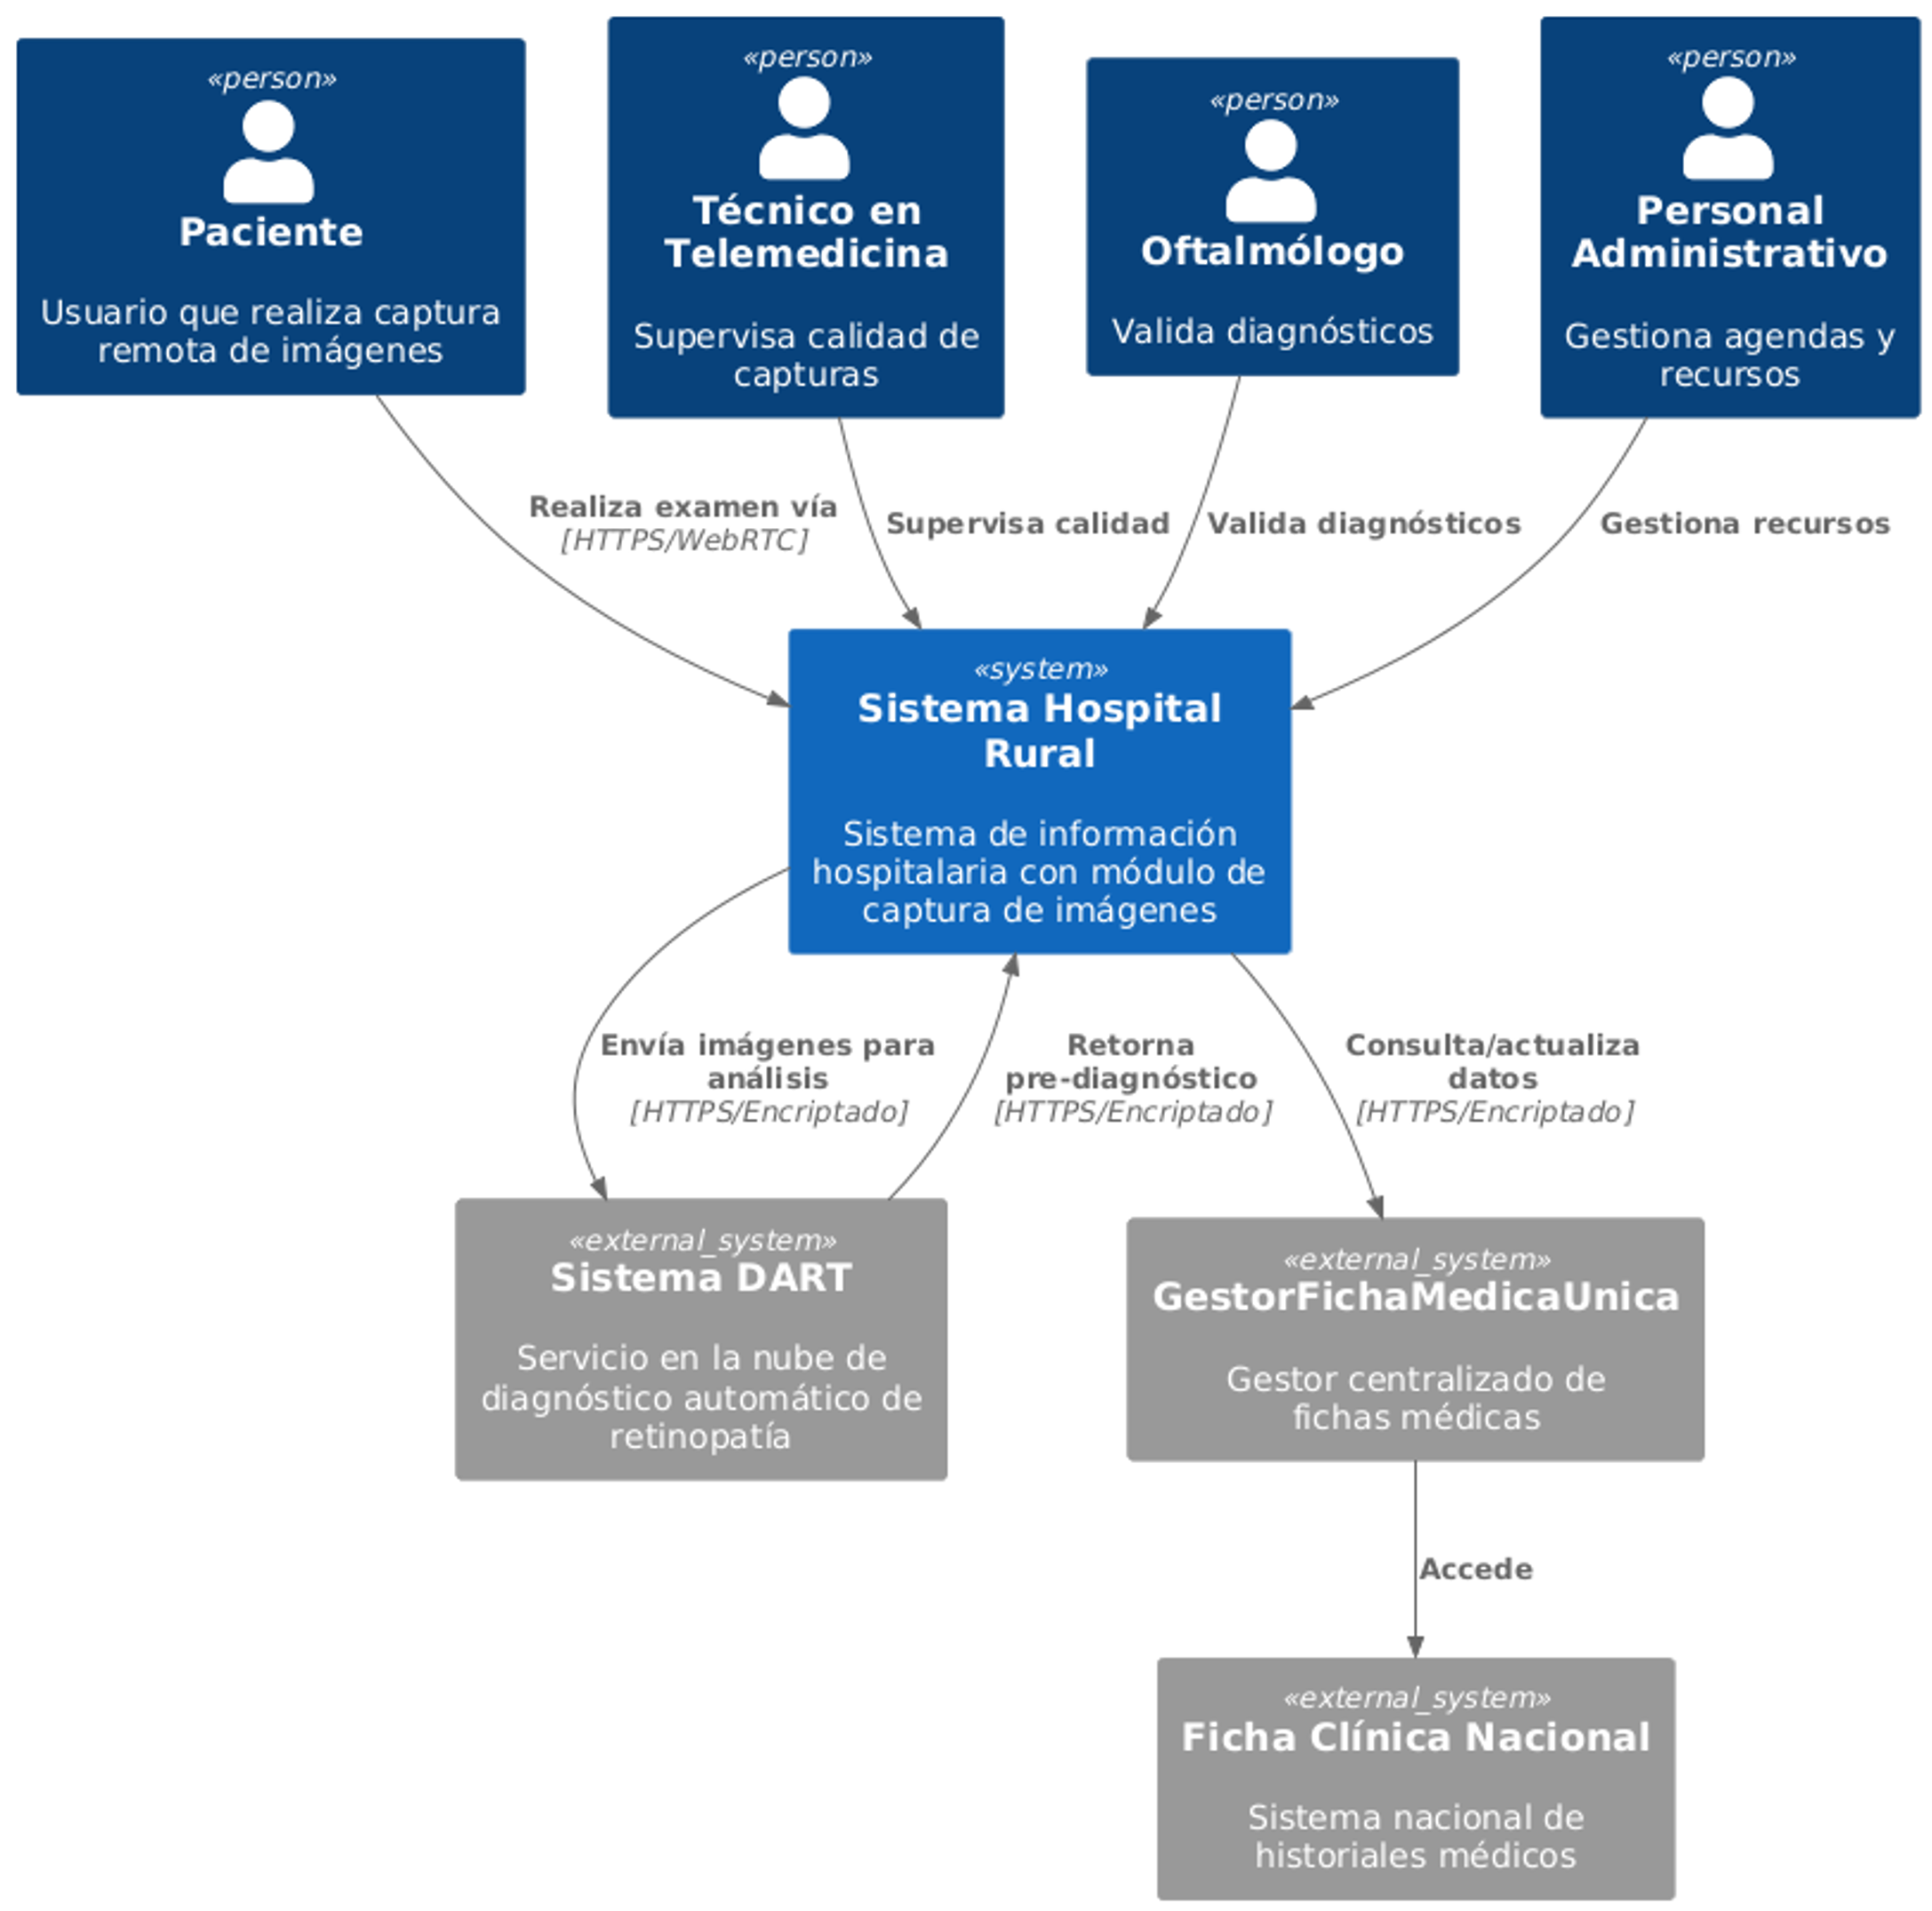
\includegraphics[width=\textwidth]{Pictures/dart_context.png}
    \caption{Diagrama de Contexto del Sistema DART integrado con el Hospital Rural}
    \label{fig:dart_context}
\end{figure}

En esta arquitectura, el Sistema de Información Hospitalaria (HIS) actúa como punto central de interacción para todos los usuarios. El paciente realiza el examen de retinopatía conectándose directamente al HIS a través de su navegador web, utilizando WebRTC para la captura de imágenes. El sistema DART, al igual que la Ficha Clínica Nacional, opera como un servicio en la nube, invisible para el usuario final. En el centro del diagrama se encuentra el Sistema DART, que interactúa con cuatro tipos de usuarios principales: el paciente, que ahora puede realizar capturas remotas de imágenes retinales; el técnico en telemedicina, que supervisa la calidad de estas capturas; el oftalmólogo, que valida los diagnósticos; y el personal administrativo, que gestiona los recursos y agendas del sistema.

La implementación utiliza tecnología WebRTC para la captura de imágenes a través del navegador, lo que elimina la necesidad de software especializado en el computador del paciente. Esta decisión arquitectónica simplifica significativamente el despliegue y la adopción del sistema, requiriendo únicamente:
\begin{itemize}
    \item Un navegador web moderno con soporte para WebRTC
    \item Una cámara web con resolución mínima de 720p
    \item Una conexión a internet estable (mínimo 1Mbps de subida)
\end{itemize}

El flujo de trabajo típico es el siguiente:
\begin{enumerate}
    \item El paciente accede al portal del hospital (HIS) para realizar su examen
    \item El HIS gestiona la captura de imágenes a través del navegador del paciente
    \item Las imágenes capturadas se envían al servicio DART en la nube para su análisis
    \item DART procesa las imágenes y retorna un pre-diagnóstico al HIS
    \item El técnico en telemedicina y/o el oftalmólogo revisan los resultados a través del HIS
    \item Una vez validado el diagnóstico, se actualiza la ficha del paciente a través del GestorFichaMedicaUnica
\end{enumerate}

Esta arquitectura distribuida ofrece varias ventajas:
\begin{itemize}
    \item Centralización de la interacción del usuario en el sistema hospitalario
    \item Procesamiento especializado en la nube mediante el servicio DART
    \item Integración transparente con los sistemas nacionales de salud
    \item Mayor seguridad al manejar datos sensibles a través de canales encriptados
\end{itemize}





\subsubsection{Paso 2: Diagrama de Contenedores}

\begin{itemize}
    \item \textbf{Descripción}: Este diagrama detalla las aplicaciones y almacenes de datos que componen el sistema DART, utilizando la notación del modelo C4. Refleja el enfoque de flujo de trabajo y muestra cómo los diferentes componentes del sistema se comunican entre sí.
    \item \textbf{Instrucciones}:
    \begin{itemize}
        \item Identificar los contenedores principales dentro del sistema hospitalario, como la Aplicación Web y la Base de Datos HIS. Los contenedores son las unidades de software que ejecutan aplicaciones o almacenan datos.
        \item Describir cómo estos contenedores se comunican entre sí y con sistemas externos, especificando las interacciones y el flujo de datos entre ellos.
    \end{itemize}
    \item \textbf{PlantUML}:
    \begin{verbatim}
    @startuml "Sistema Hospitalario"
    !include https://raw.githubusercontent.com/plantuml-stdlib/C4-PlantUML/master/C4_Container.puml

    LAYOUT_WITH_LEGEND()

    title Diagrama de Contenedores para el Sistema Hospitalario

    Person(paciente, "Paciente", "Un paciente que realiza exámenes de retinopatía")
    Person(tecnico, "Técnico en Telemedicina", "Supervisa la calidad de las capturas")
    Person(oftalmologo, "Oftalmólogo", "Valida los diagnósticos")
    Person(admin, "Personal Administrativo", "Gestiona recursos y agendas")

    System_Boundary(sistema_hospitalario, "Sistema Hospitalario") {
        Container(servidor_app, "Servidor de Aplicaciones", "Node.js, npm", "Gestiona las solicitudes de los usuarios y coordina las interacciones con otros sistemas")
        Container(spa, "Aplicación de Página Única", "JavaScript, Angular", "Proporciona toda la funcionalidad de exámenes a los pacientes a través de su navegador web")
        ContainerDb(base_datos_his, "Base de Datos HIS", "MySQL", "Almacena datos de pacientes y exámenes")
        Container(backend_api, "API de Diagnóstico", "Node.js, Docker Container", "Proporciona funcionalidad de diagnóstico a través de API")
    }

    System_Ext(servicio_dart, "Servicio DART", "Análisis de Imágenes en la Nube")
    System_Ext(ficha_clinica_nacional, "Ficha Clínica Nacional", "Sistema Externo")
    System_Ext(gestor_ficha_medica_unica, "Gestor Ficha Médica Única", "Sistema Externo")
    System_Ext(email_system, "Sistema de Correo Electrónico", "Envía notificaciones con informes adjuntos")
    System_Ext(firma_digital, "Servicio de Firma Digital", "Firma digital externa para documentos")

    Rel(paciente, spa, "Usa", "HTTPS")
    Rel(tecnico, spa, "Supervisa calidad de capturas", "HTTPS")
    Rel(oftalmologo, spa, "Valida diagnósticos", "HTTPS")
    Rel(admin, spa, "Gestiona recursos y agendas", "HTTPS")

    Rel_Neighbor(servidor_app, spa, "Entrega contenido", "HTTPS")
    Rel_Neighbor(spa, backend_api, "Usa", "async, JSON/HTTPS")
    Rel_Back_Neighbor(base_datos_his, backend_api, "Lee y escribe en", "sync, JDBC")

    Rel(backend_api, servicio_dart, "Envía imágenes para análisis", "HTTPS")
    Rel(backend_api, ficha_clinica_nacional, "Accede a datos clínicos", "HTTPS")
    Rel(backend_api, gestor_ficha_medica_unica, "Actualiza ficha médica", "HTTPS")
    Rel(backend_api, firma_digital, "Solicita firma digital", "HTTPS")
    Rel(backend_api, email_system, "Envía notificaciones con informes adjuntos", "SMTP")

    @enduml
    \end{verbatim}
    \item \textbf{Razones de Diseño}:
    \begin{itemize}
        \item \textbf{Servidor de Aplicaciones}: Gestiona las solicitudes de los usuarios y coordina las interacciones con otros sistemas.
        \item \textbf{Aplicación de Página Única}: Proporciona toda la funcionalidad de exámenes a los pacientes a través de su navegador web.
        \item \textbf{Base de Datos HIS}: Almacena de manera segura los datos de pacientes y exámenes.
        \item \textbf{API de Diagnóstico}: Proporciona funcionalidad de diagnóstico a través de API.
        \item \textbf{Sistemas Externos}: DART, Ficha Clínica Nacional, Gestor Ficha Médica Única, Sistema de Correo Electrónico y Servicio de Firma Digital son sistemas externos que interactúan con el sistema hospitalario para proporcionar servicios adicionales.
    \end{itemize}
    \item \textbf{Lectura del Diagrama}:
    \begin{itemize}
        \item Los contenedores están representados por rectángulos con el nombre del contenedor, la tecnología utilizada y su propósito.
        \item Las flechas indican el flujo de datos o solicitudes entre los contenedores y sistemas externos, con descripciones breves de las interacciones.
    \end{itemize}
\end{itemize}


\begin{figure}[h]
    \centering
    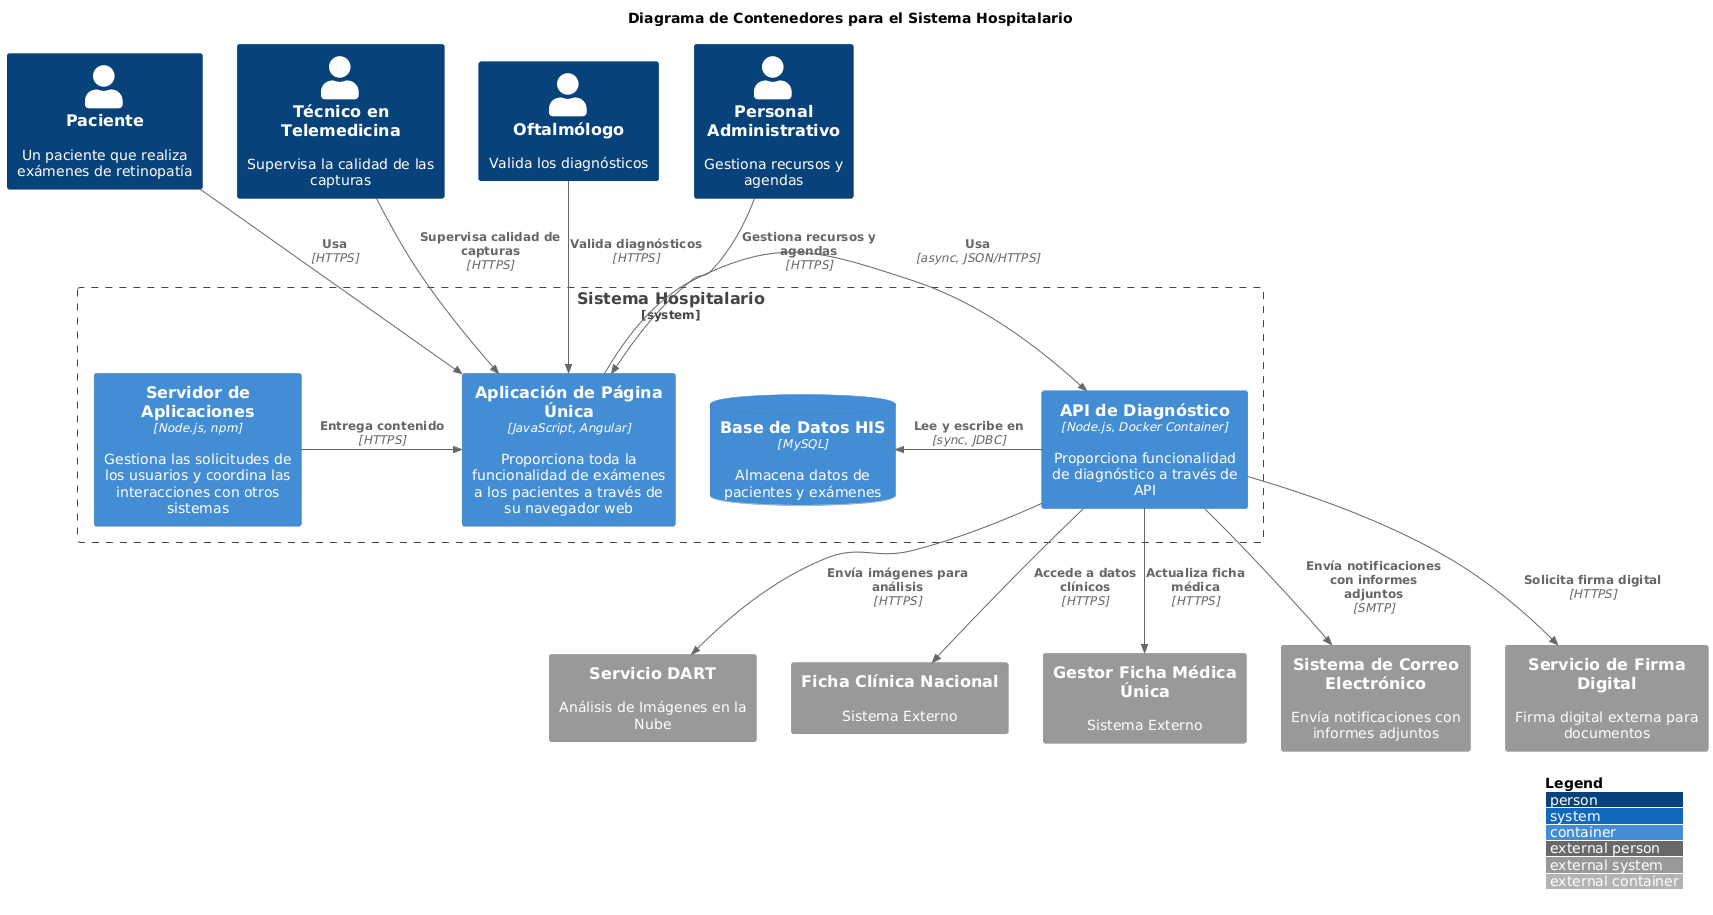
\includegraphics[width=\textwidth]{Pictures/container_diagram.png}
    \caption{Diagrama de Contenedores del Sistema Hospitalario}
    \label{fig:container_diagram}
\end{figure}










\subsubsection{Diagrama de Componentes - Explicación de los Componentes}

\begin{itemize}
    \item \textbf{Componente de Autenticación}: Gestiona la autenticación de usuarios, asegurando que solo usuarios autorizados puedan acceder al sistema.
    \item \textbf{Controlador de Exámenes}: Se encarga de la gestión de exámenes, incluyendo la creación y seguimiento de los mismos.
    \item \textbf{Generador de Informes}: Genera informes de diagnóstico que pueden ser revisados por los médicos y enviados a los pacientes.
    \item \textbf{Integración con DART}: Facilita la comunicación con el servicio DART para el análisis de imágenes.
\end{itemize}

Este diagrama detalla cómo los diferentes módulos dentro de los contenedores interactúan para proporcionar las funcionalidades del sistema. La modularidad de los componentes permite una fácil actualización y mantenimiento del sistema, mientras que la reutilización de componentes comunes mejora la eficiencia del desarrollo.


    \begin{verbatim}
    @startuml
    !include https://raw.githubusercontent.com/plantuml-stdlib/C4-PlantUML/master/C4_Component.puml

    LAYOUT_WITH_LEGEND()

    title Diagrama de Componentes para el Sistema Hospitalario

    Container(spa, "Aplicación de Página Única", "JavaScript y Angular", "Proporciona toda la funcionalidad de exámenes a los pacientes a través de su navegador web.")
    ContainerDb(base_datos_his, "Base de Datos HIS", "MySQL", "Almacena datos de pacientes y exámenes.")
    System_Ext(servicio_dart, "Servicio DART", "Análisis de Imágenes en la Nube")

    Container_Boundary(backend_api, "API de Diagnóstico") {
        Component(auth, "Componente de Autenticación", "Node.js Module", "Gestiona la autenticación de usuarios.")
        Component(exam, "Controlador de Exámenes", "Node.js Module", "Gestiona la creación y seguimiento de exámenes.")
        Component(report, "Generador de Informes", "Node.js Module", "Genera informes de diagnóstico para los pacientes.")
        Component(integration, "Integración con DART", "Node.js Module", "Facilita la comunicación con el servicio DART.")
        
        Rel(auth, base_datos_his, "Lee y escribe en", "JDBC")
        Rel(exam, base_datos_his, "Lee y escribe en", "JDBC")
        Rel(report, base_datos_his, "Lee y escribe en", "JDBC")
        Rel(integration, servicio_dart, "Envía imágenes para análisis", "HTTPS")
    }

    Rel(spa, auth, "Usa", "JSON/HTTPS")
    Rel(spa, exam, "Usa", "JSON/HTTPS")
    Rel(spa, report, "Usa", "JSON/HTTPS")

    @enduml
    \end{verbatim}
\end{itemize}
    \begin{figure}[h]
        \centering
        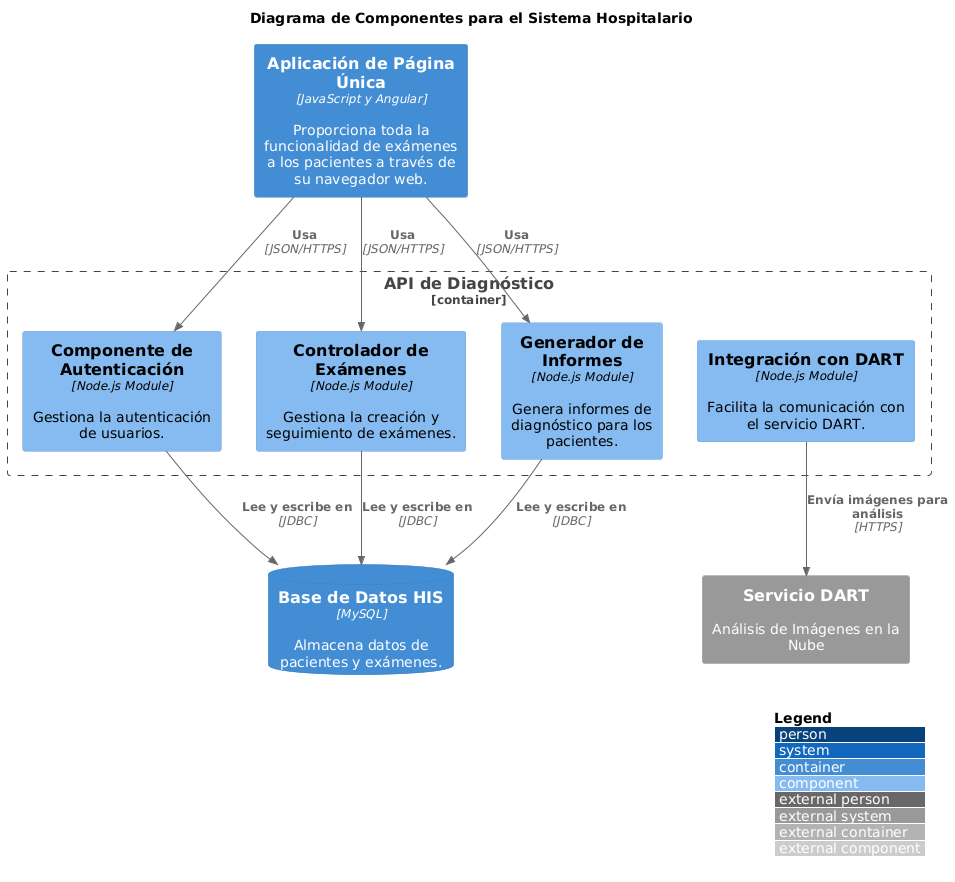
\includegraphics[width=\textwidth]{Pictures/component_diagram.png}
        \caption{Diagrama de Componentes del Sistema Hospitalario}
        \label{fig:component_diagram}
    \end{figure}























%%%%%%%%%%%%%%%%%%%%%%%%%%%%%%%%%%%%%%%%%%%%%%%%%%%
%%%%%%%%%%%%%%%%%%%%%%%%%%%%%%%%%%%%%%%%%%%%%%%%%%%
%%%%%%%%%%%%%%%%%%%%%%%%%%%%%%%%%%%%%%%%%%%%%%%%%%%
%%%%%%%%%%%%%%%%%%%%%%%%%%%%%%%%%%%%%%%%%%%%%%%%%%%
%%%%%%%%%%%%%%%%%%%%%%%%%%%%%%%%%%%%%%%%%%%%%%%%%%%
%%%%%%%%%%%%%%%%%%%%%%%%%%%%%%%%%%%%%%%%%%%%%%%%%%%
\begin{comment}
\section{Evaluación ATAM del Sistema Hospitalario con DART}

Para evaluar la arquitectura propuesta para el sistema DART, aplicaremos el método ATAM (Architecture Tradeoff Analysis Method). Este método nos permitirá analizar cómo los componentes lógicos identificados satisfacen los atributos de calidad requeridos.

\subsection{Identificación de Atributos de Calidad}

Los principales atributos de calidad para el sistema DART son:

\begin{itemize}
    \item \textbf{Desempeño}:
        \begin{itemize}
            \item Tiempo de respuesta del diagnóstico < 5 días
            \item Procesamiento de imágenes en < 1 minuto
            \item Capacidad de procesar 1000 imágenes/día
        \end{itemize}
    \item \textbf{Precisión}:
        \begin{itemize}
            \item Sensibilidad > 90\% en detección de patologías
            \item Especificidad > 85\% en clasificación
            \item Tasa de falsos positivos < 5\%
        \end{itemize}
    \item \textbf{Disponibilidad}:
        \begin{itemize}
            \item Sistema disponible 24/7
            \item Tiempo de inactividad < 1 hora/mes
            \item Recuperación automática de fallos
        \end{itemize}
    \item \textbf{Seguridad}:
        \begin{itemize}
            \item Cumplimiento de la Ley 20.584 (Derechos del Paciente)
            \item Encriptación de datos sensibles
            \item Trazabilidad completa de accesos
        \end{itemize}
\end{itemize}

\subsection{Escenarios de Atributos de Calidad}

Desarrollamos escenarios detallados para cada atributo de calidad:

\subsubsection{Escenario de Desempeño}
\begin{itemize}
    \item \textbf{Estímulo:} Llegada de 100 nuevas imágenes
    \item \textbf{Fuente:} Centro de salud rural
    \item \textbf{Artefacto:} Sistema DART completo
    \item \textbf{Entorno:} Operación normal
    \item \textbf{Respuesta:} Procesamiento y diagnóstico preliminar
    \item \textbf{Medida:} Completado en < 2 horas
\end{itemize}

\subsubsection{Escenario de Precisión}
\begin{itemize}
    \item \textbf{Estímulo:} Imagen con retinopatía moderada
    \item \textbf{Fuente:} Cámara retinal calibrada
    \item \textbf{Artefacto:} Motor de Diagnóstico IA
    \item \textbf{Entorno:} Carga normal del sistema
    \item \textbf{Respuesta:} Clasificación correcta de severidad
    \item \textbf{Medida:} Concordancia > 90\% con oftalmólogo
\end{itemize}

\subsection{Contextualización de Escenarios con 'Ilities'}

Cada escenario del sistema DART se cruza con las características de calidad relevantes, asegurando que se cumplan los objetivos de negocio:

\begin{itemize}
    \item \textbf{Escenario de Desempeño:} Procesamiento de 100 imágenes en menos de 2 horas.
    \begin{itemize}
        \item \textbf{Ilities:} Desempeño, Disponibilidad
    \end{itemize}
    \item \textbf{Escenario de Precisión:} Clasificación correcta de imágenes con retinopatía moderada.
    \begin{itemize}
        \item \textbf{Ilities:} Precisión, Seguridad
    \end{itemize}
\end{itemize}

\subsection{Análisis de Compensaciones}

Los componentes lógicos identificados presentan las siguientes compensaciones:

\begin{enumerate}
    \item \textbf{Componente de Preprocesamiento}:
        \begin{itemize}
            \item \textbf{Beneficio:} Mejora la precisión del diagnóstico
            \item \textbf{Costo:} Aumenta el tiempo de procesamiento
            \item \textbf{Riesgo:} Posible cuello de botella en alta demanda
        \end{itemize}
    
    \item \textbf{Motor de Diagnóstico IA}:
        \begin{itemize}
            \item \textbf{Beneficio:} Automatización y velocidad
            \item \textbf{Costo:} Alta complejidad de mantenimiento
            \item \textbf{Riesgo:} Dependencia de calidad de datos
        \end{itemize}
    
    \item \textbf{Sistema de Validación Médica}:
        \begin{itemize}
            \item \textbf{Beneficio:} Mayor precisión y confiabilidad
            \item \textbf{Costo:} Tiempo adicional en el proceso
            \item \textbf{Riesgo:} Disponibilidad de especialistas
        \end{itemize}
\end{enumerate}

\subsection{Análisis de Riesgos y No-Riesgos}

\subsubsection{Riesgos Arquitectónicos}
\begin{itemize}
    \item \textbf{R1:} Alto acoplamiento del Motor de IA podría dificultar actualizaciones
    \item \textbf{R2:} Dependencia de la calidad de imagen inicial
    \item \textbf{R3:} Posible degradación del rendimiento en horas pico
\end{itemize}

\subsubsection{No-Riesgos}
\begin{itemize}
    \item \textbf{NR1:} Escalabilidad del almacenamiento (uso de cloud)
    \item \textbf{NR2:} Integración con sistemas hospitalarios (APIs estándar)
    \item \textbf{NR3:} Seguridad de datos (encriptación end-to-end)
\end{itemize}

\subsection{Puntos de Sensibilidad y Compensación}

\begin{itemize}
    \item \textbf{S1:} Calidad del preprocesamiento vs. tiempo de respuesta
    \item \textbf{S2:} Automatización vs. precisión del diagnóstico
    \item \textbf{S3:} Disponibilidad vs. costos de infraestructura
\end{itemize}

\subsection{Recomendaciones Arquitectónicas}

Basados en el análisis ATAM, recomendamos:

\begin{enumerate}
    \item Implementar procesamiento por lotes para optimizar rendimiento
    \item Desarrollar un sistema de caché para resultados frecuentes
    \item Establecer un pipeline de validación automática de imágenes
    \item Implementar monitoreo continuo de precisión del modelo
    \item Diseñar un sistema de retroalimentación para mejora continua
\end{enumerate}

\section{Arquitectura del Sistema Hospitalario con DART}

\subsection{Vista de Componentes Lógicos}

La siguiente figura muestra la arquitectura de componentes lógicos del sistema hospitalario que integra DART:

\begin{figure}[h]
\begin{verbatim}
@startuml
package "Sistema Hospitalario" {
    package "DART" {
        [Adquisición de Imágenes] as AI
        [Preprocesamiento] as PP
        [Motor IA] as IA
        [Validación Médica] as VM
        [Gestor de Derivaciones] as GD
    }
    
    package "HIS (Sistema de Información Hospitalaria)" {
        [Gestión de Pacientes] as GP
        [Agenda Médica] as AM
        [Historia Clínica] as HC
        [Farmacia] as FA
    }
    
    package "Telemedicina" {
        [Portal Médico] as PM
        [Portal Paciente] as PP2
        [Gestor de Teleconsultas] as GT
    }
    
    database "Almacenamiento" {
        [Base de Datos Clínica] as BDC
        [Repositorio de Imágenes] as RI
        [Base de Conocimiento IA] as BCIA
    }
}

' Relaciones DART
AI --> PP : imágenes
PP --> IA : imágenes preprocesadas
IA --> VM : diagnóstico preliminar
VM --> GD : decisión derivación
AI --> RI : almacena
IA --> BCIA : consulta/actualiza

' Relaciones HIS
GP --> HC : actualiza
AM --> HC : registra
FA --> HC : prescripciones
HC --> BDC : almacena

' Integraciones
GP --> AI : datos paciente
VM --> HC : diagnóstico final
GD --> AM : agenda derivación
PM --> VM : acceso remoto
GT --> VM : teleconsulta
PP2 --> HC : consulta

@enduml
\end{verbatim}
\caption{Arquitectura de Componentes Lógicos del Sistema Hospitalario con DART}
\label{fig:arch_components}
\end{figure}

\subsection{Descripción de Componentes}

Los componentes se organizan en cuatro paquetes principales:

\subsubsection{DART}
\begin{itemize}
    \item \textbf{Adquisición de Imágenes}: Captura y validación inicial de imágenes retinales
    \item \textbf{Preprocesamiento}: Normalización y mejora de imágenes
    \item \textbf{Motor IA}: Análisis automatizado y detección de patologías
    \item \textbf{Validación Médica}: Interfaz para revisión y confirmación por especialistas
    \item \textbf{Gestor de Derivaciones}: Coordinación de referencias a especialistas
\end{itemize}

\subsubsection{HIS (Sistema de Información Hospitalaria)}
\begin{itemize}
    \item \textbf{Gestión de Pacientes}: Registro y administración de datos demográficos
    \item \textbf{Agenda Médica}: Programación de citas y recursos médicos
    \item \textbf{Historia Clínica}: Registro centralizado de información clínica
    \item \textbf{Farmacia}: Gestión de medicamentos y prescripciones
\end{itemize}

\subsubsection{Telemedicina}
\begin{itemize}
    \item \textbf{Portal Médico}: Acceso remoto para profesionales de salud
    \item \textbf{Portal Paciente}: Interfaz de autoservicio para pacientes
    \item \textbf{Gestor de Teleconsultas}: Coordinación de consultas remotas
\end{itemize}

\subsubsection{Almacenamiento}
\begin{itemize}
    \item \textbf{Base de Datos Clínica}: Almacenamiento estructurado de datos clínicos
    \item \textbf{Repositorio de Imágenes}: Almacenamiento especializado para imágenes médicas
    \item \textbf{Base de Conocimiento IA}: Modelos y datos de entrenamiento
\end{itemize}

\subsection{Patrones de Integración}

El diagrama muestra varios patrones de integración importantes:

\begin{enumerate}
    \item \textbf{Flujo de Trabajo DART}:
        \begin{itemize}
            \item Secuencia lineal de procesamiento de imágenes
            \item Puntos de decisión en validación médica
            \item Retroalimentación para mejora continua del modelo
        \end{itemize}
    
    \item \textbf{Integración con HIS}:
        \begin{itemize}
            \item Datos demográficos alimentan el proceso DART
            \item Resultados se incorporan a la historia clínica
            \item Derivaciones se coordinan con agenda médica
        \end{itemize}
    
    \item \textbf{Capacidades de Telemedicina}:
        \begin{itemize}
            \item Acceso remoto a diagnósticos
            \item Consultas virtuales de seguimiento
            \item Portal de autoservicio para pacientes
        \end{itemize}
\end{enumerate}

\section{Diagrama de Despliegue del Sistema Hospitalario con DART}

\subsection{Vista de Despliegue}

La siguiente figura muestra el diagrama de despliegue del sistema hospitalario que integra DART, reflejando el proceso completo:

\begin{figure}[h]
\begin{verbatim}
@startuml
node "Usuario" {
    [PC del Usuario] --> [Cámara Retinal]
}

node "Red Hospitalaria" {
    node "Servidor DART" {
        [Consulta Recibida] --> [Preprocesar Imágenes]
        [Preprocesar Imágenes] --> [Detectar Signos de Retinopatía]
        [Detectar Signos de Retinopatía] --> [Generar Propuesta de Reporte]
        [Generar Propuesta de Reporte] --> [Validación Profesional]
        [Validación Profesional] --> [Notificar Paciente]
        [Validación Profesional] --> [Petición de Intervención]
    }
    
    node "Base de Datos" {
        [Repositorio de Imágenes]
        [Base de Conocimiento IA]
    }
}

node "Interfaz de Telemedicina" {
    [Portal Médico]
    [Portal Paciente]
}

' Conexiones
[PC del Usuario] --> [Consulta Recibida] : Captura
[Generar Propuesta de Reporte] --> [Repositorio de Imágenes] : Almacenamiento
[Detectar Signos de Retinopatía] --> [Base de Conocimiento IA] : Consulta
[Validación Profesional] --> [Portal Médico] : Resultados
[Portal Paciente] --> [Validación Profesional] : Consulta

@enduml
\end{verbatim}
\caption{Diagrama de Despliegue del Sistema Hospitalario con DART}
\label{fig:deployment_diagram}
\end{figure}























\section{Evaluación de la Arquitectura}

La evaluación de la arquitectura se realiza utilizando métodos como el ATAM para asegurar que los componentes lógicos identificados satisfacen los atributos de calidad requeridos.

\begin{itemize}
    \item \textbf{ATAM (Architecture Tradeoff Analysis Method)}: Método utilizado para analizar cómo los componentes lógicos satisfacen los atributos de calidad.
    \item \textbf{Identificación de Atributos de Calidad}: Evaluar atributos como desempeño, precisión, disponibilidad y seguridad.
    \item \textbf{Escenarios de Atributos de Calidad}: Desarrollar escenarios detallados para cada atributo de calidad.
    \item \textbf{Análisis de Compensaciones}: Identificar beneficios, costos y riesgos de los componentes lógicos.
    \item \textbf{Recomendaciones Arquitectónicas}: Proponer mejoras basadas en el análisis ATAM.
\end{itemize}

\textbf{Workshop ATAM para el Piloto del Sistema DART en un Hospital}

Este workshop está diseñado para simular una evaluación ATAM en un hospital donde se implementará un piloto del sistema DART, solicitado por el Ministerio de Salud. Los participantes incluirán personal del hospital, arquitectos del sistema, y otros stakeholders relevantes.
\subsection{Objetivos del Workshop}
\begin{itemize}
    \item Evaluar la arquitectura del sistema DART en el contexto del hospital.
    \item Identificar riesgos y oportunidades de mejora.
    \item Fomentar la comunicación entre los stakeholders.
\end{itemize}

\subsection{Roles y Responsabilidades}
\begin{itemize}
    \item \textbf{Líder de Evaluación}: Facilita el proceso del workshop.
    \item \textbf{Portavoz del Proyecto}: Representante del hospital que presenta los objetivos de negocio.
    \item \textbf{Arquitecto del Sistema}: Presenta la arquitectura del sistema DART.
    \item \textbf{Stakeholders}: Incluyen médicos, personal técnico, y representantes del ministerio.
\end{itemize}

\subsection{Materiales del Workshop}
\begin{itemize}
    \item \textbf{Presentación de Diapositivas}: Guía visual para el workshop.
        \begin{itemize}
            \item \textbf{Código en Gamma para generar diapositivas}:
            \begin{verbatim}
            slide "Introducción al ATAM" {
                title: "Introducción al ATAM"
                content: "Presentación interactiva sobre el método ATAM."
            }

            slide "Presentación de Impulsores de Negocio" {
                title: "Presentación de Impulsores de Negocio"
                content: "Discusión liderada por el portavoz del proyecto."
            }

            slide "Presentación de la Arquitectura" {
                title: "Presentación de la Arquitectura"
                content: "Exposición del arquitecto del sistema."
            }

            slide "Generación del Árbol de Utilidad" {
                title: "Generación del Árbol de Utilidad"
                content: "Taller colaborativo para identificar atributos de calidad."
            }

            slide "Análisis de Enfoques Arquitectónicos" {
                title: "Análisis de Enfoques Arquitectónicos"
                content: "Evaluación de enfoques mediante discusión grupal."
            }

            slide "Lluvia de Ideas y Priorización de Escenarios" {
                title: "Lluvia de Ideas y Priorización de Escenarios"
                content: "Sesión de brainstorming con votación para priorizar escenarios."
            }

            slide "Análisis de Enfoques Arquitectónicos (Reiteración)" {
                title: "Análisis de Enfoques Arquitectónicos (Reiteración)"
                content: "Revisión de escenarios priorizados y análisis detallado."
            }

            slide "Presentación de Resultados" {
                title: "Presentación de Resultados"
                content: "Presentación final de hallazgos y recomendaciones."
            }
            \end{verbatim}
        \end{itemize}
    
    
        
    
    \item \textbf{Documentación de la Arquitectura}: Descripciones detalladas del sistema DART.
\end{itemize}

\subsection{Emulación del Workshop y Resultados Esperados}

Durante el workshop, los alumnos emularán cada paso del ATAM para obtener resultados específicos. A continuación, se describe la dinámica de cada paso, los modelos o detalles arquitectónicos presentados, y los resultados esperados, resaltados en azul.

\begin{enumerate}
    \item \textbf{Introducción al ATAM}
    \begin{itemize}
        \item \textit{Alumno (Presentador)}: Debe realizar una presentación interactiva sobre el método ATAM.
        \begin{itemize}
            \item \textcolor{blue}{Introducción al método ATAM.}
            \item \textcolor{blue}{Explicación de los pasos del proceso.}
            \item \textcolor{blue}{Importancia del método en la arquitectura de software.}
        \end{itemize}
        \item \textit{Modelo/Detalles}: Se muestra un diagrama general del proceso ATAM.
        \item \textit{Resultado}: \textcolor{blue}{Comprensión clara del método ATAM y su importancia.}
    \end{itemize}

    \item \textbf{Presentación de Impulsores de Negocio}
    \begin{itemize}
        \item \textit{Dinámica}: Discusión liderada por el portavoz del proyecto.
        \item \textit{Modelo/Detalles}: Se presentan los objetivos del Hospital 2.0, que incluyen mejorar la accesibilidad a servicios de salud, aumentar la eficiencia operativa y garantizar diagnósticos precisos y oportunos. Estos objetivos influyen en la arquitectura del servicio de diagnóstico remoto de retinopatía diabética al requerir una infraestructura tecnológica robusta, integración con sistemas existentes y un enfoque centrado en el paciente.
        \item \textit{Resultado}: \textcolor{blue}{Identificación de los impulsores arquitectónicos clave para el Hospital 2.0, tales como la mejora de la accesibilidad a servicios de salud, el aumento de la eficiencia operativa y la garantía de diagnósticos precisos y oportunos, asegurando que la arquitectura soporte los objetivos estratégicos del hospital.}
    \end{itemize}



    
    \item \textbf{Presentación de la Arquitectura}
    \begin{itemize}
        \item \textit{Dinámica}: Exposición del arquitecto del sistema.
        \item \textit{Modelo/Detalles}: Descripción detallada de la arquitectura del sistema DART, incluyendo la vista lógica y la vista física. La vista lógica muestra cómo los componentes funcionales del sistema interactúan, mientras que la vista física ilustra la infraestructura tecnológica subyacente, referenciando las figuras \ref{fig:arch_components} y \ref{fig:deployment_diagram}.
        \item \textit{Resultado}: \textcolor{blue}{Entendimiento de cómo la arquitectura soporta los objetivos de negocio. La arquitectura del sistema DART está diseñada para mejorar la accesibilidad a los servicios de salud mediante la integración con sistemas hospitalarios existentes y la provisión de diagnósticos precisos y oportunos. La vista lógica muestra cómo los componentes funcionales del sistema, como la Gestión de Pacientes y el Motor IA, interactúan para procesar y analizar imágenes médicas. La vista física ilustra la infraestructura tecnológica subyacente, incluyendo bases de datos y servidores, que asegura la disponibilidad y escalabilidad del sistema.}
    \end{itemize}

    \item \textbf{Construcción del Árbol de Utilidad}
    \begin{itemize}
        \item \textit{Dinámica}: Durante el ATAM, se lleva a cabo un taller colaborativo dirigido por el arquitecto del sistema, con la participación de todos los stakeholders clave. Se inicia con una discusión para identificar y priorizar los atributos de calidad, construyendo un árbol de utilidad que prioriza el impacto de cada atributo en los objetivos de negocio.
        \item \textit{Modelo/Detalles}: A continuación se presenta un árbol de utilidad, donde los atributos de calidad se organizan jerárquicamente según su impacto. Este esquema incluye ejemplos específicos para DART, destacando el atributo de Desempeño como prioritario.

      



        \item \textit{Resultado}: \textcolor{blue}{Clarificación de los atributos de calidad críticos, priorizando aquellos con mayor impacto en los objetivos del sistema, asegurando una comprensión común entre todos los participantes.}
    \end{itemize}

    \begin{itemize}
        \item \textbf{Desempeño}
        \begin{itemize}
            \item Latencia (H,H): Procesamiento de imágenes en menos de 1 minuto.
            \item Carga máxima (H,M): Respuesta del sistema en tiempo real.
        \end{itemize}
        \item \textbf{Disponibilidad}
        \begin{itemize}
            \item Tiempo de actividad (H,H): Sistema disponible 99.9% del tiempo.
            \item Fallo de software (M,M): Recuperación en menos de 30 segundos.
        \end{itemize}
        \item \textbf{Precisión}
        \begin{itemize}
            \item Sensibilidad (H,L): Sensibilidad > 90%.
            \item Especificidad (H,L): Especificidad > 85%.
        \end{itemize}
        \item \textbf{Seguridad}
        \begin{itemize}
            \item Encriptación (H,L): Encriptación de datos.
            \item Trazabilidad (H,L): Trazabilidad de accesos.
        \end{itemize}
        \item \textbf{Escalabilidad}
        \begin{itemize}
            \item Capacidad de usuarios (L,M): Manejo de aumento en el volumen de usuarios.
        \end{itemize}
    \end{itemize}

    \item \textbf{Análisis de Enfoques Arquitectónicos}
    \begin{itemize}
        \item \textit{Enfoque Arquitectónico}: Un enfoque arquitectónico aquí se refiere a la estrategia o método utilizado para estructurar y organizar los componentes del sistema DART, asegurando que cumpla con los requisitos de calidad y funcionalidad.
        \item \textit{Riesgos en Diagramas/Arquitecturas}: Los riesgos pueden incluir problemas como el alto acoplamiento entre componentes, lo que podría dificultar las actualizaciones o la escalabilidad del sistema.
        \item \textit{Puntos de Sensibilidad}: Estos son aspectos críticos del sistema donde pequeños cambios pueden tener un gran impacto, como la relación entre la calidad del preprocesamiento de imágenes y el tiempo de respuesta del sistema.
        \item \textit{Input para el Proceso}: Diagramas de componentes y flujos de datos del sistema DART.
        \item \textit{Salida del Proceso}: Plantillas que documentan los riesgos identificados y los puntos de sensibilidad.
        \item \textit{Ejemplo en DART}:
        \begin{itemize}
            \item \textbf{Riesgo}: Dependencia excesiva del Motor IA en la calidad de las imágenes preprocesadas podría afectar la precisión del diagnóstico.
            \item \textbf{Punto de Sensibilidad}: Equilibrio entre la automatización del diagnóstico y la precisión requerida.
        \end{itemize}
        \item \textit{Resultado}:
        \begin{itemize}
            \item \textbf{Riesgos Identificados}:
            \begin{itemize}
                \item \textbf{Riesgo 1}: Dependencia excesiva del Motor IA en la calidad de las imágenes preprocesadas.
                \item \textbf{Riesgo 2}: Alto acoplamiento entre componentes que podría dificultar actualizaciones.
            \end{itemize}
            \item \textbf{Puntos de Sensibilidad}:
            \begin{itemize}
                \item \textbf{Punto de Sensibilidad 1}: Equilibrio entre la automatización del diagnóstico y la precisión requerida.
                \item \textbf{Punto de Sensibilidad 2}: Relación entre la calidad del preprocesamiento de imágenes y el tiempo de respuesta del sistema.
            \end{itemize}
        \end{itemize}
    \end{itemize}

    \item \textbf{Lluvia de Ideas y Priorización de Escenarios}
    \begin{itemize}
        \item \textit{Dinámica}: Sesión de brainstorming con votación para priorizar escenarios.
        \item \textit{Modelo/Detalles}: Listado de escenarios y su impacto en la arquitectura, utilizando los modelos C4.
        \item \textit{Ejemplos de Escenarios}:
        \begin{itemize}
            \item \textbf{Escenario 1}: Integración del Sistema DART con el Sistema de Información Hospitalaria para la transferencia de datos de pacientes.
            \item \textbf{Escenario 2}: Escalabilidad del Sistema DART para manejar un aumento en el volumen de usuarios durante campañas de salud pública.
            \item \textbf{Escenario 3}: Implementación de medidas de seguridad para proteger los datos de los pacientes en el Sistema DART.
            \item \textbf{Escenario 4}: Optimización del tiempo de respuesta del Motor de Diagnóstico IA bajo diferentes condiciones de carga.
        \end{itemize}
        \item \textit{Resultado}: \textcolor{blue}{Priorización de escenarios críticos para el análisis, asegurando que estén alineados con los modelos C4.}
    \end{itemize}

    \item \textbf{Análisis de Enfoques Arquitectónicos (Reiteración)}
    \begin{itemize}
        \item \textit{Dinámica}: Revisión de escenarios priorizados y análisis detallado.
        \item \textit{Modelo/Detalles}: Revisión de diagramas y modelos de arquitectura.
        \item \textit{Resultado}: \textcolor{blue}{Identificación de cambios necesarios en la arquitectura para abordar los escenarios. Por ejemplo, se podría descubrir la necesidad de un nuevo componente de seguridad para proteger los datos de los pacientes, lo cual llevaría a modificar la arquitectura existente.}
    \end{itemize}

    \item \textbf{Presentación de Resultados}
    \begin{itemize}
        \item \textit{Dinámica}: Presentación final de hallazgos y recomendaciones.
        \item \textit{Modelo/Detalles}: Resumen visual de los resultados del ATAM.
        \item \textit{Resultado}: \textcolor{blue}{Documentación de riesgos, no-riesgos, y recomendaciones arquitectónicas.}
    \end{itemize}
\end{enumerate}

\subsection{Resultados Esperados}
En conclusión, a lo largo de este curso hemos aprendido los fundamentos del diseño arquitectónico, la importancia de un método sistemático y los conceptos de diseño y drivers arquitectónicos. También hemos estudiado las características de calidad según ISO/IEC 9126 y el proceso de diseño arquitectónico. 

Aplicamos estos conocimientos al sistema DART del MINSAL, identificando componentes lógicos y patrones de acoplamiento, y utilizando el modelo C4 para construir la arquitectura del hospital con DART. Realizamos una evaluación detallada de la arquitectura del sistema en el contexto del hospital, identificando riesgos y oportunidades de mejora, y fomentando la comunicación entre los stakeholders.

Los resultados de nuestro análisis incluyen específicamente la identificación de dos riesgos críticos: la dependencia excesiva del Motor IA en la calidad de las imágenes preprocesadas y el alto acoplamiento entre componentes que podría dificultar actualizaciones. También se identificaron oportunidades de mejora en la escalabilidad del sistema y en la implementación de medidas de seguridad para proteger los datos de los pacientes. Además, se clarificaron los requisitos de calidad, como la precisión del diagnóstico y el tiempo de respuesta del sistema, y se mejoró la documentación de la arquitectura, detallando los componentes y sus interacciones. Estos resultados son esenciales para el éxito del sistema y proporcionan una base sólida para futuras referencias y desarrollos. Además, hemos logrado una comunicación efectiva entre los stakeholders, lo cual es vital para la colaboración y el alineamiento de objetivos.

\end{comment}




\section{Referencias}

\begin{itemize}
    \item Cervantes, H., Kazman, R. (2016). Designing Software Architectures: A Practical Approach, 2nd Edition. Addison-Wesley Professional.
    \item Gandhi, R., Richards, M., Ford, N. (2023). Head First Software Architecture: A Learner's Guide to Architectural Thinking. O'Reilly Media.
\end{itemize}

